\documentclass[11pt,a4paper]{article}
\usepackage[T1]{fontenc}
\usepackage{lmodern}
\usepackage{amsmath,amssymb,amsthm}
\usepackage[margin=2.5cm]{geometry}
\usepackage{graphicx}
\usepackage{pgfplots}
\pgfplotsset{compat=1.18}
\usepackage{xcolor}
\usepackage{booktabs}
\usepackage{tabularx}
\usepackage{longtable}
\usepackage[export]{adjustbox}
\usepackage{enumitem}
\usepackage{microtype}
\usepackage[section]{placeins}
\usepackage[colorlinks=true,linkcolor=blue!55!black,citecolor=blue!55!black,
            urlcolor=blue!55!black,bookmarks=true,bookmarksnumbered=true,
            unicode=true]{hyperref}

\widowpenalty=10000
\clubpenalty=10000
\emergencystretch=3em
\numberwithin{equation}{section}

\theoremstyle{plain}
\newtheorem{theorem}{Theorem}[section]
\newtheorem{lemma}[theorem]{Lemma}
\newtheorem{corollary}[theorem]{Corollary}
\newtheorem{proposition}[theorem]{Proposition}
\newtheorem{conjecture}[theorem]{Conjecture}
\theoremstyle{definition}
\newtheorem{definition}[theorem]{Definition}
\newtheorem{example}[theorem]{Example}
\theoremstyle{remark}
\newtheorem{remark}[theorem]{Remark}

\newcommand{\Z}{\mathbb{Z}}
\newcommand{\R}{\mathbb{R}}
\newcommand{\T}{\mathbb{T}}
\newcommand{\floor}[1]{\left\lfloor #1 \right\rfloor}
\newcommand{\wn}[1]{\lVert #1 \rVert_{N}}
\newcommand{\wnc}[1]{\lVert #1 \rVert}
\newcommand{\lrc}{\mathrm{LRC}}
\newcommand{\taust}{\mathrm{TAU}}
\DeclareMathOperator{\ord}{ord}
\DeclareMathOperator{\cls}{cls}
\DeclareMathOperator{\Vol}{Vol}

\graphicspath{{./}}

\newcommand{\papertitle}{Every Natural Strengthening Examined Is False: Type Mismatch
in Lossless Reformulations of the Lonely Runner Conjecture}

\hypersetup{
  pdftitle={\papertitle},
  pdfauthor={Anonymous},
  pdfsubject={Lonely Runner Conjecture; reformulations; covering radius;
              zonotopes; Ehrhart theory; negative results},
  pdfkeywords={Lonely Runner Conjecture, lossless reformulation,
               type mismatch, covering radius, LR-zonotope, Ehrhart
               h*-polynomial, arithmetic matroid, exact witnesses,
               branch and bound certification}
}

\begin{document}

\title{\papertitle}
\author{Anonymous}
\date{Version 6.0}
\maketitle

\tableofcontents
\clearpage

% ======================================================================
% Section 1 — Abstract and Introduction
% ======================================================================

\begin{abstract}
\noindent
The Lonely Runner Conjecture ($\lrc_n$) admits many \emph{lossless}
reformulations---finite, geometric, dynamical, or arithmetic rewrites that
are exactly equivalent to it. This paper is about a structural fact that
emerged from a multi-year program of attacking the conjecture through such
reformulations: \emph{every natural strengthening of a lossless
reformulation that the program examined---every version of it that would
open a new toolkit---is false}. The claim is an observational summary of
four witnessed settings, not a meta-theorem over all conceivable
strengthenings. A reformulation equivalent to $\lrc$ carries the full
truth-content of $\lrc$; a strictly stronger version is false, and the
falsity is visible at small $n$ with exact rational witnesses. We exhibit
the type mismatch in four settings across two reformulation worlds. The
finite pair-sum covering reformulation supports three of them: its proved
inventory, audited statement-by-statement, contains only closure,
invariance, and exhaustiveness statements (no proved margin-type statement
exists in it); its single margin-shaped instrument, a transfer-matrix
model of the solution cascade, is closed by theorem \emph{in its
single-anchor scope} (the constrained transfer matrices are partial
permutations with spectral radius exactly $0$ or $1$; the general
branching strand-census operator is not covered by the theorem); and its
character-rigidity route has orbit-invariance laws falsified exactly, with
marginal envelopes saturated precisely where the missing margin would be
needed. The fourth setting is independent of the
cascade: the Lonely Runner zonotope, whose covering radius satisfies a
strictly stronger inequality than $\lrc$ that is false from $n=5$ on,
with the exact value $\rho=16/47>1/3$ at
$v=(1,2,3,4,5)$ (certified from both sides by branch and bound) and
$\rho\ge17/47>5/14$ at $v=(1,2,3,4,5,12)$ (a rational witness at a
certified argmax, superseding every earlier record), strict exact
witnesses $\rho\ge
29/80>5/14$ at $v=(1,2,3,4,5,6)$, $\rho\ge 4/11>5/14$ at
$v=(1,2,3,4,5,7)$, and $\rho\ge 1793/5000>5/14$ at $v=(1,2,3,4,5,9)$,
and a proved weight identity among the quotient norm's pair forms that
forces the denominators of the exact values (the recurring $47$ is
$3\cdot4+3\cdot5+4\cdot5$), while its
Ehrhart $h^*$-polynomials are real-rooted and log-concave through
$n=10$ (verified by exact Sturm sequences) with strictness decaying like
$\Theta(1/n)$ in the measured range and no statistically distinguishable
correlation with covering margins at the achievable sample sizes.
Alongside the negative result the paper states the program's one bounded positive
theorem---the sum-only equality $M(V)=\max_{\{u,w\}}\tau(u,w)$, the
rigid-zone translate-class classifications at the primes
$7,11,13,17,19,37$, and the composite-side structure at $p^2$ and $pq$,
stated with their hypothesis ledger---and a finite witness archive with a
certification ladder: exact deepest-hole classification at $n=3$,
independent away-certified and branch-and-bound certificates at $n=4$
(including $v=(1,2,3,16)$, $\rho=9/34$), exact refutations at
$n=5,6$---the sharpest with a two-sided certificate, the second at a
certified argmax point---and, from an independent
branch-and-bound method,
certified deepest-hole equality at $n=5$, $m=10,20,25,30$
($\rho=\delta$ exactly at each; $m=10$ closed with an exact Lipschitz
box certificate after its first attempt stranded on a residual of volume
below $6\times10^{-7}$). Every number cited in this abstract is
re-asserted by a persisted, independent, exact computation (a 225-item
ledger with zero failures, and a seven-witness cross-validation of the
incorporated certification records, zero failures), and the certification
method carries a negative control that correctly refuses a false
statement.
The paper is a negative-results paper and claims no progress on the
conjecture itself: it proves no new cases of $\lrc$, and the surviving
equivalent forms are as hard as they ever were. What it contributes is the
obstruction's anatomy: why four natural toolkits, each correct and each
productive on its own terms, cannot cross the same gap.
\end{abstract}

\section{Introduction}\label{sec:intro}

\subsection{The conjecture and the reformulation habit}

Let $n\ge 2$ and let $V=(v_1,\dots,v_n)$ be distinct positive integers
with $\gcd(V)=1$ ($n$ moving runners plus the stationary observer; the
instances of this paper have $n\ge 3$, the range where the quotient
geometry of \S\ref{sec:prelim} is nondegenerate). Runners start together
at the origin of the unit circle
$\T=\R/\Z$; runner $p$ occupies $v_p t \bmod 1$ at time $t$. Write
$\wnc{x}$ for the distance of a real number to the nearest integer. The
\emph{loneliness} of the stationary observer at time $t$ is
$g(t)=\min_{1\le p\le n}\wnc{v_p t}$, and $M(V)=\max_{t\in\T}g(t)$. The
Lonely Runner Conjecture, posed by Wills in 1967 and independently by
Cusick in the language of view obstruction
\cite{PS-survey,Wills,Cusick1973}, asserts $M(V)\ge 1/(n{+}1)$ for every
$V$. It is proved for up to fifteen runners: the classical cases
$n\le7$ \cite{PS-survey}, eight runners \cite{Rosenfeld8}, nine and ten
\cite{Trakulthongchai}, eleven through thirteen \cite{Sungkawichai}, and
fourteen and fifteen \cite{Allikvere}; beyond fifteen only computational
verifications of special families are known
\cite{PS-survey,MSS}.

Attacking such a conjecture through equivalent rewrites is an old habit.
The reformulation landscape around the Lonely Runner problem is unusually
rich: Wills' original inhomogeneous-approximation form; Cusick's view
obstruction; Rifford's continuous covering problem in dimension $n-2$,
equivalent to a time-bound version of the problem \cite{Rifford}; and, from
the program this paper reports on, a finite form---the pair-sum lattice
reduction---under which the conjecture becomes a family of covering
statements about explicit cyclic groups \cite{PS-survey,prog-artifacts}.
Each rewrite is \emph{lossless}: it holds exactly when $\lrc_n$ holds,
with no residual error term. Each was adopted in the hope that its native
toolkit---covering combinatorics, spectral theory, harmonic analysis,
polyhedral geometry, Ehrhart theory---could move the conjecture.

This paper records, in a form we hope is useful beyond this one problem,
what that hope runs into. The headline is a sharp negative observation,
exhibited in four settings across two reformulation worlds:

\begin{quote}
\emph{LRC admits many lossless reformulations, and every natural
strengthening of them that this program examined and exhibited---every
reformulation that would open a new toolkit---is false. This is not a
limitation of one technique; it is a structural pattern, documented in
four settings (three manifestations of the pair-sum cascade and one
zonotope--Ehrhart setting) with finite exact witnesses.}
\end{quote}

The three cascade settings are not independent experiments: they are three
probes of the same reformulation (an inventory audit, an instrument
closure, and a rigidity falsification), and the paper counts them
separately only because each fails for a different reason. Independent of
the cascade is the fourth setting, the zonotope; the paper's claim is the
pattern across both worlds, not four unrelated facts. The pattern claim
is deliberately larger than the paper's evidence: four documented
instances from one program are one thread's worth of confirmation,
offered as a case study of a structural law that should hold verbatim in
any comparable reformulation culture---lossless equivalence preserves
hardness exactly, and the natural strengthenings fail where they matter.
The thread's specific contributions are the pair-character identity of
\S\ref{sec:witness} (a small, proved, exact law that governs the
arithmetic of the deepest holes) and the certified archive around it;
the walls themselves are the general phenomenon.

The mechanism, which we call \emph{type mismatch} and develop in
\S\ref{sec:tm}, has three faces. First, losslessness transfers truth
exactly: a proof of the reformulated statement is ipso facto a proof of
$\lrc$, and conversely. A rewrite may still change tractability---the
program's own finitization is an equivalent rewrite that made the problem
computable instance by instance---but it cannot discard the conjecture's
content, and no lossless rewrite can be simultaneously strictly stronger
than $\lrc$ and true at the extremal instances. Second, the statements
that would make a reformulation tractable---a uniform margin, a spectral
gap, a saturated bound with slack, a monotone scale law---are strictly
stronger than $\lrc$ (they imply it; the converse fails); at the extremal
instances the extra margin they demand does not exist, and they are false
there with exact witnesses. Third, the instruments that a lossless
reformulation naturally supports (classifications, invariances, exact
counts) compose into statements of the wrong type: they close everything
except the one gap that matters. All four settings were probed by exact
computation, and the witnesses are small, checkable, and archived
(\S\ref{sec:witness}, Appendices~\ref{sec:prov} and \ref{sec:self}).

\subsection{The four instances in one paragraph each}

\emph{Instance 1: the finite covering reformulation}
(\S\ref{sec:tm-covering}). The pair-sum equality theorem reduces
$M(V)$ exactly to a maximum over cyclic groups $\Z_{v_u+v_w}$
(\S\ref{sec:positive}), turning $\lrc_n$ into a covering question about
explicit bad sets. The program's classification toolkit (size laws, moat
counts, class-group reductions, lift laws) closed $75.6\%$ of a
$3{,}712{,}576$-instance corpus outright and localized the rest to one
named class---but a statement-by-statement audit of the full proof
inventory found \emph{zero} proved statements of the missing type (a
uniform growth-in-$k$ margin over a trivial baseline); every proved
statement is a closure, invariance, exhaustiveness, or machine
verification, and the one candidate that reads like an exception (the cut
law's ``$k$-cancellation'') is a $k$-\emph{invariance}---the exact
opposite of a growth-in-$k$ margin.

\emph{Instance 2: the transfer-matrix route} (\S\ref{sec:tm-transfer}).
The single instrument shaped to produce the missing type---a
transfer-matrix or automaton model of the solution cascade, whose natural
output is a spectral quantity uniform in scale---was executed as a proof
attempt under a pre-committed success criterion and closed by theorem
\emph{in its single-anchor scope}: every single-anchor constrained
transfer matrix of the lossless cascade is a partial
permutation with spectral radius exactly $0$ or $1$; the cyclic product is
diagonal, its trace is the survivor count itself, and at the six
reflection-symmetric committed families the survival fraction is exactly
$1$ forever. The general branching strand-census operator is not covered
by the theorem and is left open. Losslessness forbids generated decay
for the single-anchor operator: bijections preserve
measure, deletion filters without dissipating, and the single-anchor
reformulation is bounded by its own fidelity.

\emph{Instance 3: character rigidity} (\S\ref{sec:tm-char}). The
harmonic-analytic route phrased the obstruction in terms of a closed
system of ten characters. Its natural strengthenings---orbit-invariance
of singleton or pairwise marginal profiles---are \emph{false}, falsified
by exhaustive exact computation; the marginal envelope saturates (is
full) exactly at the configurations where the margin is needed, and the
only invariant sparsity is joint. The trivial bound sits exactly at the
cascade threshold: beating it by the factor the obligations require
($\sim\!250$ at every rung) is precisely the open margin, stated twice.

\emph{Instance 4: the Lonely Runner zonotope}
(\S\ref{sec:tm-zono}). The quotient torus $\R^n/(\R v+\Z^n)$ carries a
covering radius $\rho(v)$ in the quotient $\ell_\infty$ norm, and the
Lonely Runner statement for the center class is
$\delta(v)\le (n{-}1)/(2(n{+}1))$ with $\delta\le\rho$ always. The
covering-radius form---\emph{every} hole within the threshold, not just
the center---would open the geometry-of-numbers toolkit. It is false from
$n=5$: at the extremal harmonic instance $v=(1,2,3,4,5)$ the covering
radius is exactly $\rho=16/47>1/3$ (a two-sided certificate), at
$v=(1,2,3,4,5,12)$ there is an argmax-certified point at $17/47>5/14$,
at $v=(1,2,3,4,5,6)$ one at
$29/80>5/14$, at the non-extremal $v=(1,2,3,4,5,7)$ one at
$4/11>5/14$, and at $v=(1,2,3,4,5,9)$ one at $1793/5000>5/14$. Meanwhile the Ehrhart $h^*$-polynomials of the zonotopes
are beautifully behaved---real-rooted, log-concave, Newton, uniformly,
through $n=10$ in both core families---but their strictness decays like
$\Theta(1/n)$ and has no measurable correlation with the covering
margins: the coefficient-level toolkit cannot see the metric hole depth
at all.

\subsection{What this paper is and is not}

The paper is deliberately plain about its shape. It is a \emph{sharp
negative result}---a whole class of approaches to a famous problem, and
the exact reason each fails---plus \emph{one bounded positive theorem}
carried over from the companion monograph (the equality theorem, the
rigid-zone classifications, and the $p^2$/$pq$ composite structure,
\S\ref{sec:positive}) and a \emph{finite witness archive} with an explicit
certification ladder (\S\ref{sec:witness}). Negative results of this kind
are genuinely valuable when they come with exact computational evidence
and a mechanism; the mechanism here (losslessness versus strengthening)
applies verbatim to any problem with a comparable reformulation culture.

The boundary of the claims is as follows. The paper does not solve,
reduce, or weaken the Lonely Runner Conjecture; no new cases of $\lrc$
are proved at any $n$; the rung results of
\cite{Rosenfeld8,Trakulthongchai,Sungkawichai,Allikvere} are untouched.
The equivalent forms that survive our audits (the $\delta$-form of the
covering statement, the pair-sum formulation) are exactly as hard as
$\lrc$, and we claim no leverage on them. The falsified strengthenings
are stronger than $\lrc$ by construction, so their falsity implies
nothing about $\lrc$ itself---which remains open, tight at the harmonic
instances, and apparently indifferent to every toolkit this program could
bring to bear. What the archive adds is certainty about where \emph{not}
to dig: four doors, each closed by exact computation or by theorem, each
closing for the same reason.

\subsection{Roadmap and conventions}

\S\ref{sec:prelim} fixes notation and the four equivalent forms of the
covering statement, with the proofs of equivalence deferred to the
companion monograph where they are long. \S\ref{sec:tm} states the
type-mismatch mechanism and develops the four instances.
\S\ref{sec:positive} summarizes the positive core with exact statements.
\S\ref{sec:witness} presents the witness archive and the certification
ladder, including the exact value $\rho=16/47$ (certified from both
sides), the argmax-certified $17/47$, the closed ladder row $m=10$
($\rho=7/22=\delta$), and
the weight identity that governs their denominators.
\S\ref{sec:concl} concludes. Appendix~\ref{sec:hstar} records the
$h^*$-observations (the extension to $n=9,10$ is included here).
Appendix~\ref{sec:prov} is the provenance ledger: every number cited in
this paper is re-asserted by independent exact computation in a
persisted, machine-checkable run (225 items, zero failures), and the
certification scripts, budgets, and outputs are listed.
Appendix~\ref{sec:self} is the self-contained verification core: the
elementary identity behind the four forms, the runner formulation with
its Lipschitz certificate, the explicit pair-sum statement of
Theorem~\ref{thm:equality}, and one-line hand checks of the headline
witnesses, so that a reader with only this paper can verify the sharpest
negative claims without the companion monograph.

All computations are exact (rational arithmetic) unless explicitly marked
as a float enclosure; the one exception class is flagged where it occurs
(numerical root finding is supplemented by exact Sturm-sequence
verification, and the statistical statements carry their sample sizes and
$p$-values). Certification levels are labeled \emph{exact}
(complete exact proof), \emph{certified} (complete proof with an
independent numerical outer loop), or \emph{consistent} (search-level
evidence only), following the ladder of \S\ref{sec:prelim}
\cite{prog-artifacts}.

% ======================================================================
% Section 2 — Preliminaries
% ======================================================================

\section{Preliminaries}\label{sec:prelim}

\subsection{Notation}

Throughout, $n\ge 3$ is the number of speeds, $V=(v_1,\dots,v_n)$ has
distinct positive integer entries with $\gcd(V)=1$ and $v_1=1$ when a
coordinate model is in use, and $\wnc{x}=\min(x-\floor{x},
\floor{x}+1-x)$ is the distance to the nearest integer. For a modulus
$N$ we write $\wn{x}:=\min_{j\in\Z}|x-jN|$ for the distance from $x$ to
the nearest multiple of $N$ (so $\wn{x}=N\,\wnc{x/N}$). We write
$\lambda(V)=\max_{t\in\T}\min_p \wnc{v_p t}$ for the optimal loneliness
and $M(V)$ for the same quantity; the two notations are interchangeable
and we keep $\lambda$ in metric contexts and $M$ in the
pair-sum context. The threshold is
$\mathrm{thr}_n=(n-1)/(2(n+1))=1/2-1/(n+1)$. Two speed families recur:
the \emph{harmonic} family $V=(1,2,\dots,n)$ and the \emph{rung-2}
family $V=(1,\dots,n-1,2n)$. For these, $\lambda$ is classical:
$\lambda(1,\dots,n)=1/(n+1)$ exactly (the harmonic family is extremal,
with zero margin against the conjecture), and
$\lambda(1,\dots,n-1,2n)=2/(2n+1)$ exactly (the rung-2 family is not
extremal; its margin is $1/((n+1)(2n+1))$). Both identities are
re-asserted exactly for $n\le 10$ in the provenance run of
Appendix~\ref{sec:prov}.

\subsection{Four forms of the covering statement}

Write $\delta(V)=\tfrac12-\lambda(V)$ and let $\mathbf{1}=(1,\dots,1)$.
The following forms of $\lrc_n$ are used interchangeably in the
literature and in this program, and it is essential to keep their
strengths apart.

\begin{enumerate}[leftmargin=1.6em,itemsep=2pt]
\item \textbf{Loneliness form.} $\lambda(V)\ge 1/(n+1)$ for all $V$.
\item \textbf{Center-depth form ($\delta$-form).}
$\delta(V)\le \mathrm{thr}_n$, where
$\delta(V)=\operatorname{dist}_\infty\!\bigl(\R v,\;\Z^n+\tfrac12\mathbf{1}\bigr)$
is the $\ell_\infty$ distance from the trajectory line to the shifted
lattice. The identity
$\delta=\tfrac12-\lambda$ is elementary: for every $t$,
$\max_j \wnc{\tfrac12-v_jt}=\tfrac12-\min_j\wnc{v_jt}$.
\item \textbf{Quotient-torus form.} Let $\mathcal{X}_v=\R^n/\R v$ be
the quotient vector space (the calligraphic symbol avoids colliding with
the speed vector $V$), let $\pi\colon\R^n\to\mathcal{X}_v$ be the
projection, $\Lambda=\pi(\Z^n)\cong\Z^{n-1}$, and let
$\|\cdot\|_{\mathcal{X}_v}$ be the quotient norm
$\|c\|_{\mathcal{X}_v}=\operatorname{dist}_\infty(x,\R v)$ for any lift
$x$ of $c$. Then $\delta(V)=\operatorname{dist}_{\mathcal{X}_v}(c^*,\Lambda)$
where $c^*=\pi(\tfrac12\mathbf{1})$ is the \emph{center class}, a
$2$-torsion point whose coordinates are $\tfrac12$ on even speeds and $0$
on odd speeds. The $\delta$-form reads: the center class has quotient-norm
depth at most $\mathrm{thr}_n$ in every $\mathcal{X}_v$.
\item \textbf{Covering-radius form ($\rho$-form).}
Let $\rho(V)=\max_{c\in\mathcal{X}_v}\operatorname{dist}_{\mathcal{X}_v}(c,
\Lambda)$ be the covering radius of $\Lambda$ in the quotient norm. The
$\rho$-form of the conjecture asserts $\rho(V)\le\mathrm{thr}_n$ for all
$V$.
\end{enumerate}

Forms (1)--(3) are equivalent to $\lrc_n$: this is the content of the
shift identity above together with the standard quotient-torus dictionary,
and the equivalence is asserted computationally, exactly, on every
instance of the program (the geometric pipeline is validated end to end
in the runs of Appendix~\ref{sec:prov}). Form (4) is \emph{strictly
stronger}. Since the maximum defining $\rho$ ranges over all classes and
$\delta$ is the depth of one class, $\delta(V)\le\rho(V)$ always; hence
$\rho\le\mathrm{thr}_n$ implies the $\delta$-form and thus $\lrc_n$. The
converse fails, and the failure is not an artifact of small examples: it
begins exactly at $n=5$ and persists (\S\ref{sec:tm-zono},
\S\ref{sec:witness}). At the harmonic instances the $\delta$-form is
tight ($\delta=\mathrm{thr}_n$), so the $\rho$-form has no slack to
absorb the difference between the center and the deepest hole: the
two statements coincide on all tested instances for $n\le 4$---more
precisely, the $\rho$-form \emph{holds} on every instance tested at
$n\le 4$, certified through $m=24$ at $n=3$ and $m=16$ at $n=4$, while
the center-is-deepest property holds exactly at the multiples---which is
why the identification was easy to believe---and separate from $n=5$ on,
with exact witnesses.

For computations we use two further standard facts, both proved and
machine-validated in the program's records \cite{prog-artifacts}. First,
in \emph{$c$-coordinates} $c_j=x_j-v_jx_1$ ($j=2,\dots,n$; valid when
$v_1=1$) the lattice is exactly $\Z^{n-1}$ and the quotient norm is the
maximum of the finitely many linear forms
\[
\phi^{1j}=\frac{c_j}{1+v_j},\qquad
\phi^{ij}=\frac{v_jc_i-v_ic_j}{v_i+v_j}\quad(2\le i<j),
\]
each of $\ell_1$-norm at most $1$; hence
$\|c\|_{\mathcal{X}_v}\le\|c\|_\infty$ and Lipschitz certification
needs no norm-equivalence constant. Second, the depth function admits the
one-parameter \emph{runner formulation}
\begin{equation}\label{eq:runnerform}
D(c)\;=\;\min_{\sigma\in[0,1)}\;\max\Bigl(\wnc{\sigma},\;
\max_{j\ge 2}\wnc{c_j-v_j\sigma}\Bigr),
\end{equation}
which is the distance of $c$ to $\Lambda$ on the quotient torus; this is
the form used by the branch-and-bound certifier of \S\ref{sec:witness},
and it was validated against the independent linear-form/lattice-search
implementation on random rational points for every instance used in this
paper (forty points per instance, exact agreement throughout).

\subsection{The Lonely Runner zonotope and its Ehrhart theory}

The \emph{LR-zonotope} of $V$ is $Z(V)=\pi([0,1]^n)\subset
\mathcal{X}_v$; it is an $(n{-}1)$-dimensional lattice zonotope with
respect to $\Lambda$, with relative volume $\sum_j v_j$ (normalized
volume $d!\,\sum_j v_j$, so that $h^*(1)=d!\,\sum_j v_j$)
\cite{Shephard,BeckRobins}. Its lattice-point geometry encodes the
covering problem above: holes of the $\Lambda$-covering correspond to
classes of large quotient depth. Its Ehrhart theory is arithmetic and
clean \cite{BeckRobins,dAMoci,StanleyEC}. Writing $d=n-1$, the Ehrhart
polynomial of $Z(V)$ is
\begin{equation}\label{eq:ehr}
\mathrm{Ehr}_{Z(V)}(t)\;=\;\sum_{k=0}^{d} e_k\,t^k,\qquad
e_k\;=\;\sum_{\substack{S\subseteq[n]\\|S|=k}}\gcd\!\bigl(v_{S^c}\bigr),
\qquad e_d=\sum_j v_j,
\end{equation}
and the $h^*$-polynomial is obtained
from the Eulerian expansion
$\sum_{t\ge0}\mathrm{Ehr}(t)z^t=h^*(z)/(1-z)^{d+1}$; explicitly
$h^*(z)=\sum_k e_k\,(1-z)^{d-k}A_k(z)$ with $A_k$ the Eulerian
polynomials in the shifted convention $A_0=1$, $A_1=z$, $A_2=z+z^2$
(so $A_k(z)=\sum_{j}\left\langle{k\atop j}\right\rangle z^{j+1}$ for
$k\ge1$) \cite{Frobenius}. Formula \eqref{eq:ehr} was derived in the
program's records and verified in three independent ways on every
instance used here (the Eulerian expansion, the standard Ehrhart
inversion, and a depth-first coset count at $t=1,2$;
Appendix~\ref{sec:prov}). The gcd structure is that of the arithmetic
matroid of the projected basis \cite{dAMoci}, which is why the
arithmetic-matroid literature is the natural home for the residual
positive question in Appendix~\ref{sec:hstar}.

\subsection{The certification ladder}

Every classification claim in this paper carries one of three labels.
\emph{Exact}: a complete proof in rational arithmetic (the $d=2$
arrangement enumerations; all refuting witnesses, which are single
evaluations of $D$ at rational points). \emph{Certified}: a complete
proof in which an outer numerical loop (a grid or a branch-and-bound
frontier) is combined with an exact inner analysis and a rigorous
one-sided error bound (the $d=3$ away-certifications; the
branch-and-bound certificates of \S\ref{sec:witness}). \emph{Consistent}:
search-level evidence only (grid maxima equal to the claimed value,
multi-start optimization finding nothing above it), with no completeness
claim. The labels exist precisely because enclosure-level evidence must
not be presented as proof; the ladder is applied uniformly to every
claim in this paper.

% ======================================================================
% Section 3 — The type-mismatch mechanism and four instances
% ======================================================================

\section{The type-mismatch mechanism and four instances}\label{sec:tm}

\subsection{The mechanism}\label{sec:tm-mech}

Call a statement $R$ a \emph{lossless reformulation} of $\lrc_n$ if $R$
holds for all speed vectors at rung $n$ if and only if $\lrc_n$ does, with
no slack in either direction. Call a statement $S$ a \emph{toolkit
strengthening} of $R$ if (i) $S$ implies $R$, strictly, and (ii) the
strictness is of the kind that a named toolkit can exploit: a uniform
margin over a trivial baseline, a spectral gap, an interior rate, a
monotone law in the scale parameter, a saturated bound with slack. The
distinction is not aesthetic; it is the difference between statements
that classification, spectral, harmonic, or polyhedral instruments can
consume and statements they cannot.

Three observations, jointly verified four times in this program, make up
the mechanism.

\begin{enumerate}[leftmargin=1.6em,itemsep=2pt]
\item \textbf{Losslessness transfers truth exactly.} A proof of the
reformulated statement is ipso facto a proof of $\lrc_n$, and conversely.
A rewrite may still change tractability---the program's own finitization
is an equivalent rewrite that made the problem computable instance by
instance---but it cannot discard the conjecture's content: no lossless
rewrite can be simultaneously strictly stronger than $\lrc_n$ and true
at the extremal instances.
\item \textbf{The strengthening is false where it matters.} The
toolkit-relevant strengthenings are strictly stronger than $\lrc$ (they
imply it; the converse fails), and at the extremal instances (the
harmonic and rung-2 families, the reflection-symmetric cascade families,
the tight covering configurations) the extra margin they demand does not
exist. When the demand is a definite statement, it is false, and small
$n$ exhibits the falsity with exact witnesses.
\item \textbf{The instruments land on the closed side.} The instruments a
lossless reformulation naturally supports---exact counts,
classifications, invariances, exhaustiveness checks---compose into
statements that close everything \emph{except} the missing margin: by
theorem in Instance 2 (Lemma~\ref{lem:monomial}), by audit in Instance 1
(the inventory classification), and by measurement in Instances 3 and 4
(the saturation and decay records below).
\end{enumerate}

The four subsections that follow develop one instance each. Three of
them sit on the same pair-sum cascade (an inventory audit, an instrument
closure, a rigidity falsification) and the fourth is independent of it
(the zonotope); what is common to all four is the mechanism, and we
state it once, here, as the paper's organizing claim: \emph{in each
setting, the falsity or unavailability of the strengthening is not an
accident of the example but a consequence of the losslessness that made
the reformulation faithful.}

\subsection{Instance 1: the finite covering reformulation}\label{sec:tm-covering}

The pair-sum equality theorem (\S\ref{sec:positive}) reduces
$M(V)$ to a finite maximum over cyclic groups: $M(V)=\max_{\{u,w\}}
\tau(u,w)$, where $\tau$ is the optimal loneliness on the pair-sum
lattice of denominator $N=v_u+v_w$. Under this reduction $\lrc_n$
becomes the statement that for every $V$ some pair's bad sets
$B_p=\{k\in\Z_N:(n{+}1)\wn{v_pk}<N\}$, $p\in[n]\setminus\{w\}$, fail to
cover $\Z_N$: a finite covering problem, exact, and apparently made for
the covering toolkit.

The toolkit delivered. The program proved an exact size law for the bad
sets, a polygonal witness lemma, moat-counting and coincidence-counting
lemmas, a lift law, and a class-group reduction at prime moduli; it
classified the unit covering configurations completely at the rigid
primes (Theorem~\ref{thm:rigid}); and on the full corpus of
$3{,}712{,}576$ primitive $5$-sets with speeds $\le 56$ it closed
$75.6\%$ of instances by proved lemmas alone ($78.2\%$ with the
coincidence lemma) and all of them by per-modulus verification,
localizing the residual obstruction to a single named class
\cite{prog-artifacts}. What it did not deliver, at any point in the
program's multi-year run, is a single statement of the type the residual
obstruction requires: a \emph{uniform growth-in-$k$ margin over a trivial
or measured baseline}.

This is a verifiable claim, and it was verified by audit: the full proof
inventory of the program---$34$ named results across the pair-sum,
group-ring, tensor, and cascade sections---was classified
statement-by-statement. Every proved statement is a closure, an
invariance, an exhaustiveness, or a machine verification. The one
candidate that reads like an exception, the cut law's
``$k$-cancellation,'' resolves as a $k$-scale \emph{invariance} of the
composed bound: it cancels exactly the $k$-dependence that a margin
would need to grow---the opposite of the missing type. The
spacing/packing lemma, the chain-class volume law, and the dilate theorem
were each examined as potential margin carriers and each resolves the
same way: a $k$-growing \emph{count} whose margin over its own trivial
baseline is $k$-free, a degrading order-factor slack, or a conditional
consequence of the hypothesis stack it was meant to prove.

The empirical half of the reading (``no proved margin-type statement
exists in the inventory'') is thereby settled. The structural half (``no
classification toolkit \emph{can} produce one'') is a hypothesis about
tool reach; it is what Instances 2--4 test, in three independent
settings, and what the falsity archive of \S\ref{sec:witness} completes
on the metric side.

\subsection{Instance 2: the transfer-matrix route, closed by theorem}
\label{sec:tm-transfer}

The one margin-shaped candidate instrument in the entire program was a
transfer-matrix (automaton) model of the solution cascade: transfer
operators naturally emit spectral quantities uniform in the scale
parameter, and a uniform spectral gap would be exactly the missing type.
The route was built under a success criterion fixed before computing:
the whole-cascade survival fraction must be bounded by
$\rho^{\mathrm{depth}}$ times the initial mass, with spectral radius
$\rho\le 1-\epsilon$ and $\epsilon$ independent of scale.

\begin{lemma}[Monomial dichotomy; Lemma M of the program records, single-anchor scope]
\label{lem:monomial}
Every constrained transfer matrix of the lossless cascade \emph{that
tracks a single anchor placement along the drift} is a partial
permutation matrix. Its spectrum is $\{0\}$ together with roots of unity;
its spectral radius is exactly $0$ or $1$, never interior, at any scale.
The affine pair maps compose to the identity
around any closed fiber loop (the dilation ratios telescope), so the
cyclic transfer product is diagonal, and its trace is the cascade's own
survivor count.
\end{lemma}

The proof is short once the state space is fixed: the cascade is
non-consuming (pure intersection semantics), the drift maps are
bijections, and a bijection constrained to an invariant subset is a
partial permutation. \emph{The scope is load-bearing}: the theorem
covers the single-anchor operator only; the general strand-census
operator scans the complement interval position by position with
\emph{branching} local coverage states, is not a partial permutation,
and may have interior spectral radius (the $2\times2$ witness below,
radius $1.122$). The general case is left open; the single-anchor
dichotomy is what is established. The machine record is not short:
$1500/1500$ random constrained systems; $12{,}000$ exact trace
fingerprints over $300$ systems; $66$ homogenized pair systems on the
committed families, with
spectral radius $1$ at exactly the six reflection-symmetric families
(their deletion sets close into $2$-cycles and the two-fiber survival
fraction is exactly $1.0000$ at all depths) and $0$ at the other sixty
(total extinction within three iterates, the intermediates set by lattice
runs of solution points, not by geometric decay). The criterion is
unattainable by theorem for the single-anchor operator, not merely
unattained.

Two further doors were checked. Coarse-grained or weighted automata can
carry interior spectral radii numerically, but the radius dominates every
cycle's geometric mean, so a uniform gap would force uniform decay of the
census weights---the margin as an \emph{input}, not an output---and the
converse fails (a $2\times2$ witness with all cycle means $\le0.9$ and
radius $1.122$: branching resurrects). Averaged or randomized operators
collapse to the independent-extension baseline. And the reduction closes
the loop: the whole-cascade survival fraction equals the product of
consecutive conditional ratios, each bounded by the pair-volume and
solution-set thinness hypotheses the route was commissioned to prove. The
instrument is the census in different notation; it consumes the
hypotheses it was built to generate. Losslessness forbids generated
decay \emph{for the single-anchor operator}---bijections preserve
measure, deletion filters without dissipating---and the single-anchor
reformulation is bounded by its own fidelity. The general branching
strand-census operator is not covered and is left open.

\subsection{Instance 3: character rigidity and saturated envelopes}
\label{sec:tm-char}

The harmonic-analytic route phrased the cascade obstruction in terms of
\emph{characters}: the four singleton coordinates and six pairwise
differences of the placement vector form a closed system of ten
functionals (Lemma C10 of the program records), closed under the
renormalization action up to affine shifts, whose aggregate
marginal-multiset is an orbit invariant. Any class-level census law must
live on this system; the route's natural strengthenings are laws about
its per-character profiles.

They are false, exactly. The singleton-profile orbit invariance (Lemma
V$'$) fails at both fully-enumerated primes: per-key counts match across
orbit members only after a size permutation, and the profiles differ. The
pairwise-profile invariance (V$''$) fails with $0/32$ sigma-matched
tuples. The mechanism is \emph{anchor mixing}: the renormalization
bijection couples every moving slot to the anchor coordinate; slot
singletons map to anchor pairs and pairwise differences to non-anchor
singletons, so no per-character statistic can be invariant---only the
aggregate is.

Worse, the per-character envelopes are \emph{saturated} exactly where the
margin would be needed. On the committed top orbits the pinning envelope
equals the modulus at both $k=2$ primes and $27/29$ at $k=3$ (fullness
fractions $1.000$, $1.000$, $0.931$): the marginal boxes are full, the
$\gamma$-envelope sits at or above the threshold value $4$ at $k=2$, and
the only invariant sparsity is \emph{joint} (median joint densities in
the marginal box: $1.5\%$, $7.4\%$, $6.9\%$). A bound phrased on
individual characters is tight---zero slack---precisely at the
configurations the obligations target.

Finally, the trivial bound sits exactly at the cascade threshold. The
baseline $|Sol|\le p^{m-1}$ realizes the constant
$c_1=(T/(T-6)+o(1))^{m-1}$ (here and below $m=T-3$ is the arc count of
the frontier cell, so $m-1=T-4$)---numerically $256$, $243$, $244.14$ at
$T=8,9,10$---which is exactly the value at which the depth denominator
of the conditional scaling theorem vanishes. The hypothesis H1g's
content is to beat the trivial bound by a factor growing in $k$; the
measured factors ($95\times$, $1{,}207\times$, $3{,}803\times$ at
$k=2,3,4$) grow, but the first of them starts \emph{below} the
threshold constant ($95<244$, the $k=2$ factor against the $T=10$
threshold $c_1=244.14$), which is precisely why the margin must
grow in $k$ and why $k=2$ alone cannot certify anything; the proved
factors do not exist, and the sharp-constant question and the margin
question are one criterion stated twice. This is the type mismatch in its purest
form: the character system is exactly rich enough to locate the
obstruction and exactly too poor to bound it.

\subsection{Instance 4: the Lonely Runner zonotope}\label{sec:tm-zono}

The fourth instance is metric, and its falsity archive is the paper's
sharpest. The quotient-torus model of \S\ref{sec:prelim} gives two
statements: the $\delta$-form (the center class is within
$\mathrm{thr}_n$ of the lattice), which is equivalent to $\lrc_n$, and
the $\rho$-form (every class is), which is strictly stronger and would
open the geometry-of-numbers toolkit---transference bounds, covering
radius inequalities, dilution arguments. The natural lemma a
covering-radius toolkit wants first is exactly $\rho\le\mathrm{thr}_n$.

It is false, with exact witnesses, from $n=5$, and the two sharpest
witnesses carry certified argmax structure. At the extremal harmonic
instance $v=(1,2,3,4,5)$ the deepest hole has the exact depth
\[
\rho\;\ge\;\frac{16}{47}\;>\;\frac13=\mathrm{thr}_5,
\]
attained at the rational point
$c=(\tfrac{122}{1175},\tfrac{688}{1175},\tfrac{284}{1175},
\tfrac{80}{1175})$, whose deepest-hole structure binds four pair forms
of the quotient norm under a weight identity that forces the denominator
(\S\ref{sec:weights}): the deepest hole is not the center, and the
covering-radius statement fails at the very instance where the
$\delta$-form is tight. At $n=6$ the harmonic witness
$c=(0,\tfrac5{16},\tfrac{15}{16},\tfrac34,\tfrac12)$ gives
$D=29/80>\tfrac5{14}=\mathrm{thr}_6$, and the non-extremal instance
$v=(1,2,3,4,5,7)$---whose center depth is the \emph{computed}
$\delta=1/3$, strictly below $\mathrm{thr}_6$ with slack---carries
$c=(\tfrac1{16},\tfrac9{16},0,\tfrac38,0)$
with $D=4/11>\mathrm{thr}_6$: the falsity is not an extremal-curiosity
confined to the tight family, and the covering-radius failure there is
not an artifact of center-class tightness. The rung-2 instance
$v=(1,2,3,4,5,12)$ has the exact witness $\rho\ge17/47>\mathrm{thr}_6$,
attained at
$c=(\tfrac{4714}{5875},\tfrac18,\tfrac58,\tfrac6{25},
\tfrac{2034}{5875})$ (its earlier recorded witness sat at exactly
$5/14=\mathrm{thr}_6$, a zero-slack boundary case that separated the
deepest hole from the center, $\delta=9/26<5/14$, without strictly
exceeding the threshold; the new witness upgrades it to a strict
refutation), and the instance $v=(1,2,3,4,5,9)$, which sits at the
threshold from the center side ($\delta=5/14$ computed), carries the
strict witness $\rho\ge 1793/5000>\mathrm{thr}_6$. All witnesses are
non-torsion points---the deepest holes are
not the center classes---and all are single exact evaluations of
\eqref{eq:runnerform}, checkable by hand (Appendix~\ref{sec:self}).

For $n\le4$ the $\rho$-form holds on every instance tested: at $n=3$
the deepest-hole property (that the maximum of $D$ is attained at the
center class) holds exactly when $3\mid m$ in the family
$(1,2,m)$ for $m\le24$, and at $n=4$ it holds when $4\mid m$ for
$m\le16$ (away-certified at $m=4,8,12$; branch-and-bound certified at
$m=16$, \S\ref{sec:bb}), with exact witnesses against every other $m$.
The two forms have the same truth value throughout the tested small
range---which is precisely why the stronger form was tempting; the
$n=5$ witness is precisely why it is wrong.

The companion hope---that the zonotope's Ehrhart theory could control
the covering radius through the positivity structure of its
$h^*$-polynomial---fails independently, and its failure mode is the
cleanest illustration of type mismatch in the whole program. The
The $h^*$-polynomials are real-rooted, log-concave, and Newton, uniformly,
in every instance tested through $n=10$ in both core families
(Appendix~\ref{sec:hstar}). But the log-concavity \emph{strictness} $S$
decays roughly like $30/n$ in the measured range ($nS$ drifting from
$\approx37$ to $\approx30$ in the harmonic family over
$n=3,\dots,10$, and from $60.5$ to $\approx30$ in the rung-2 family),
and Newton's inequalities force $S$ above a floor $\approx1+4/d$ that
itself declines, so much of the decay is generic and the $1/n$ behavior
cannot persist indefinitely---there is no growing quantitative margin to
spend; and across the instance sweeps the strictness has no
statistically distinguishable correlation with the covering margins at
the achievable sample sizes (Spearman $+0.32$, $p=0.32$, $N=12$ at
$n=3$; $-0.31$, $p=0.45$, $N=8$ at $n=4$; the sign flip is consistent
with noise; these arrays are too small to establish correlation or its
absence). A
coefficient inequality of a counting polynomial at growing scale $t$ is
the wrong type to pin a fixed-scale metric hole depth; the computation
says so twice, once by decay and once by the absence of a measurable
signal, and the covering-radius statement it was meant to feed is false
at the extremal instances anyway. There is no mechanism, and none is
needed: the bridge is dead on both ends.

\subsection{The pattern}

Table~\ref{tab:instances} assembles the four instances. Each row names
the reformulation, the toolkit strengthening it wanted, the status of
that strengthening, and the witness. The rows are independent; the last
column is always finite, exact, and small. We emphasize what the table
does \emph{not} contain: any statement falsifying $\lrc$ itself, or any
statement weakening our certainty that the surviving equivalent forms
(the $\delta$-form, the pair-sum form) are exactly as hard as the
original.

\begin{table}[htbp]
\centering
\small
\caption{The four instances of type mismatch. ``Margin type'' is the
statement class the toolkit needed; ``status'' is its verified fate,
with the kind of verification distinguished: \emph{false} (an exact
witness falsifies a definite statement), \emph{closed by theorem} (a
theorem shows the instrument cannot produce the output), and
\emph{zero in inventory} (an audit finding: no statement of the type
exists among the proved results). The first three rows sit on the same
pair-sum cascade; the fourth is the independent zonotope setting.}
\label{tab:instances}
\begin{tabularx}{\textwidth}{@{} l >{\raggedright\arraybackslash}X
>{\raggedright\arraybackslash}X l @{}}
\toprule
Reformulation & Toolkit wanted & Status & Witness \\
\midrule
Pair-sum covering & growth-in-$k$ margin & zero in inventory (audit;
$34$ statements); $k$-cancellation is a $k$-invariance & audit record
($34$ statements) \\
Transfer cascade & spectral gap $1-\epsilon$ & closed by theorem
(Lemma~M; survival $=1$ at reflection families) & six families, exact \\
Character rigidity & per-character profile laws & false (V$'$/V$''$
witnesses); envelopes saturated; trivial bound at threshold &
exhaustive orbits; $0/32$ \\
LR-zonotope & $\rho\le\mathrm{thr}_n$ (covering) & false from $n=5$;
$h^*$ strictness decays, no measurable signal & $16/47$, $17/47$
(argmax), $29/80$, $4/11$, $1793/5000$ (exact) \\
\bottomrule
\end{tabularx}
\end{table}

% ======================================================================
% Section 4 — The positive core
% ======================================================================

\section{The positive core: classification at the rigid primes and at
\boldmath$p^2$/$pq$}\label{sec:positive}

The program's attacks were launched from a positive base, and that base
survives the negative results intact. This section states it with
precision; the full proofs, the verification records, and the
measurement methodology are the subject of the companion monograph
\cite{prog-artifacts}, and nothing here improves or weakens them. What
matters for this paper's thesis is that the positive core is exactly as
bounded as it is: everything it proves is a closure, classification, or
identity, and its one conditional theorem wears its hypotheses on its
sleeve.

\subsection{The sum-only equality theorem}

The analytic folklore (recorded in a comment on Tao's weblog
\cite{Tao-blog}) is that the optimal time is rational with denominator
the sum or difference of two speeds. The sharpening the program proved
is that \emph{sums alone suffice}.

\begin{theorem}[Sum-only equality; Theorem 1.1 of the companion
monograph]\label{thm:equality}
Let $V=(v_1,\dots,v_n)$ have distinct positive entries with
$\gcd(V)=1$ and $0<M(V)<\tfrac12$. For each unordered pair $\{u,w\}$
let $\tau(u,w)$ denote the optimal loneliness of the $(n-1)$-runner
instance obtained by restricting to the pair-sum lattice of denominator
$N=v_u+v_w$---explicitly (Appendix~\ref{sec:self}),
\[
\tau(u,w)\;=\;\max_{k\in\Z_{N}}\;\min_{p\in[n]\setminus\{w\}}
\wnc{\tfrac{v_pk}{N}}
\]
(runners $u$ and $w$ coincide on the lattice, since
$\wnc{v_uk/N}=\wnc{v_wk/N}$ there). Then
\[
M(V)\;=\;\max_{\{u,w\}}\tau(u,w),
\]
and consequently $\lrc_n$ holds for all $V$ if and only if the finite
statement $(\taust_n)$ does: for every $V$, some pair-sum lattice
carries an optimal value $\ge 1/(n+1)$. The finitization is exact; no
information is lost, and nothing about the classical difficulty is
claimed to become easier.
\end{theorem}

The two ingredients are that the binding runners at a global optimum can
be chosen two-sided, forcing the optimal time onto a \emph{sum} lattice
(difference denominators never carry the optimum), and a mirror lemma:
on that lattice the two binding runners are exact reflections of each
other at every lattice time, so the $n$-runner minimum there equals an
$(n-1)$-runner minimum. The equivalence of Corollary form
($\lrc_n\iff\taust_n$) is the lossless gateway through which every
instance of \S\ref{sec:tm-covering} entered.

\subsection{The covering framework and the rigid zone}

Under the equality theorem, a pair \emph{certifies} an instance unless
its $n-1$ bad sets $B_w=\{k\in\Z_N:(n{+}1)\wn{wk}<N\}$ cover $\Z_N$.
The framework that follows is finite and exact, and its proved pieces
include a size law for the bad sets, a polygonal witness lemma, moat
counting, a coincidence-counting lemma, a lift law, and a class-group
reduction at prime moduli (Lemma 2.2--2.7 of the companion
monograph). Five empirically distinct obstruction classes from the
program's early experiments collapse, in this language, into additive
orders of one covering phenomenon.

\begin{theorem}[Rigid-zone classifications; Theorems 3.1--3.5 of the
companion monograph]\label{thm:rigid}
At rung $n=4$ the unit-capable moduli---those $N$ for which $n-1$ unit
bad sets can cover $\Z_N$---are $7,11,13$; at rung $n=5$ they are
$7,13,17,19,37$ within the verified range (primes $\le150$, composites
$\le111$). At every one of these primes the covering configurations are
classified completely by a short explicit list of translate classes in
the cyclic group: antipodal classes and domino tilings at $7$ and $11$;
perfect matchings at $13$; the classes $\{0,1,2,7\}$, $\{0,2,4,6\}$ at
$17$ and $19$ (together with one further class at $19$); and the single
class $\{0,2,12,15\}$ at $37$.
\end{theorem}

This is the program's central structural finding: \emph{at rigid primes,
the covering obstruction is governed by a small translate-class
structure}, and the classification is what closes $75.6\%$ of the
$3{,}712{,}576$-instance corpus outright. The residual obstruction is
localized (mixed order signatures at composite moduli), and the composite
side carries the structure that the next subsection records.

\subsection{The composite side: group ring, tensor, and the fiber
cascade}

Beyond the unit capable moduli, at $N=p^2$ and $N=pq$, the program built
the composite-side structure that the scaling question lives on. The
group-ring translation expresses the covering count as a cyclotomic
coefficient problem; the $pq$ side decomposes as a tensor problem whose
Lam--Leung-type structure \cite{LamLeung} fixes the admissible
fiber-count signatures; and the foot-count input to the cascade was
discharged by an exact identity verified on $10{,}410$ triples with the
fixed threshold at $p=31$. The higher rungs carry a general-$T$ fiber
machinery, an exact dilate-intersection lemma, a reflection-fiber
invariance, a chain-class dilate theorem, and a renormalization lemma;
the Mirsky--Newman covering-system theorem and the
R\'edei--de Bruijn--Schoenberg structure theorem for vanishing sums of
roots of unity \cite{MirskyNewman,LamLeung} play the classical
supporting roles.

Everything above is proved and machine-verified. What is \emph{not}
proved is the scaling closure itself, and the program consolidated it
into a single conditional statement with a disclosed ledger.

\begin{theorem}[Conditional scaling closure; Theorem 5.1 of the
companion monograph, $\pm$-reduced]\label{thm:SC}
Assume the multi-fiber survivor inequality Hq$_\pm$ (with additive error
term), the distinct-family volume law H1g, and the resonance zone cutoff
H2r of the companion's ledger. Then the fiber cascade over the
$\pm$-representative fiber set $U_\pm$ empties the frontier cell
$(1K,T{-}3U)$ of every rung $T\ge8$ at $N=p^2$, within a depth that is
$O_T(\log k)$ (explicit leading term $\log k/\log(T/(T-6))$); no
$k$-uniform linear bound is claimed, and the earlier ``$\le T+3$'' is
withdrawn. The reduction chain and every other input are proved or
machine-validated; each constant's provenance---derived, measured, or
fitted, with the data it is fit to---is disclosed in the six-entry
hypothesis ledger, and the open obligations are reduced to named objects:
the strand census (for H1g), the sharp pair-line constants (for H2m), and
the zone cutoff $\Lambda_0$ (for H2r). Cell emptiness is a covering
statement only; it does not by itself imply $\mathrm{LRC}$ at the rung.
\end{theorem}

We do not restate the ledger here. Its relevance to this paper is its
shape: the proved side of the ledger is all closures and identities; the
open side is exactly the growth-in-$k$ margins whose type-mismatch
career occupies \S\ref{sec:tm}. Theorem~\ref{thm:SC} is what the positive
core amounts to when stated at its exact strength, and it is why the
program's claim to a positive result is deliberately the bounded one:
\emph{the obstruction is completely classified where classification
suffices, and the residual is a named margin of a type no turn of the
program ever proved}.

% ======================================================================
% Section 5 — The witness archive
% ======================================================================

\section{The witness archive}\label{sec:witness}

The archive has four shelves: exact refutations of the covering-radius
form (each a single rational point, checkable by one evaluation of
\eqref{eq:runnerform}, the sharpest carrying a complete two-sided
certificate---the exact covering radius itself), the arithmetic law
that governs the denominators of the
exact values (\S\ref{sec:weights}), the deepest-hole certification
ladder for the family $(1,\dots,n{-}1,m)$, and the branch-and-bound
certificate method together with its negative-control validation. Every
entry is re-asserted by two independent exact implementations in the
provenance run of Appendix~\ref{sec:prov}.

\subsection{Exact refutations of the covering-radius form}

Table~\ref{tab:refute} lists the witnesses. Each witness $c$ is a
rational point of the quotient torus in $c$-coordinates; the claimed
value is $D(c)$ from \eqref{eq:runnerform}, computed exactly and
independently by the linear-form/lattice-search implementation of the
program's records. The first entry carries the strongest certification
in the archive: the value $16/47$ is the covering radius itself,
certified from both sides---the witness below, and the branch-and-bound
upper certificate of \S\ref{sec:bb}, whose tree empties at $r=16/47$.
The second entry is \emph{argmax-certified}: the displayed value is
not merely attained at the witness point but is the maximum of $D$ on
the whole argmax neighborhood, certified exactly by the arrangement
analysis of \S\ref{sec:bb} (all vertices, ridges, and corners of the
region evaluated in rational arithmetic), and the argmax carries the
binding structure of \S\ref{sec:weights} that forces the denominator;
its global equality remains open (\S\ref{sec:bb}).
The harmonic instance is extremal for the $\delta$-form
($\delta=\mathrm{thr}_n$ exactly), so the value $16/47$ kills the
$\rho$-form at the very instance where the surviving equivalent form is
tight; the rung-2 instance $v=(1,2,3,4,5,12)$ was previously a
boundary row (witness value exactly $\mathrm{thr}_6$) and is now a
strict refutation; the $m=9$ row is upgraded from boundary to strict
witness; the $v=(1,2,3,4,5,6)$ and $v=(1,2,3,4,5,7)$ rows are strict
witnesses of long standing. The witnesses are non-torsion in every
case: the deepest holes are not the center classes.

\begin{table}[htbp]
\centering
\footnotesize
\caption{Exact witnesses against the covering-radius form
$\rho(V)\le\mathrm{thr}_n$. All values are exact rational lower bounds
for $\rho$; the first is \emph{exact-certified} (the branch-and-bound
tree empties at $r$ equal to the displayed value, so the value is the
covering radius itself), the second \emph{argmax-certified} (the
maximum of $D$ on the whole argmax neighborhood equals the displayed
value, exact arrangement analysis); both are depths of the deepest
hole, not merely point depths. Witness points are in $c$-coordinates
(\S\ref{sec:prelim}). ``$>\mathrm{thr}$?'' marks whether the value
\emph{strictly} exceeds the threshold: only strict rows falsify the
$\rho$-form; boundary rows (equality) separate the deepest hole from
the center class without falsifying it. The $\delta$ entries for
non-harmonic instances are computed values, not harmonic identities.}
\label{tab:refute}
\begin{tabularx}{\textwidth}{@{} l l l >{\raggedright\arraybackslash}X l c @{}}
\toprule
$V$ & $\delta=\tfrac12-\lambda$ & $\mathrm{thr}_n$ & witness $c$ &
$\rho$ & $>\mathrm{thr}$? \\
\midrule
$(1,2,3,4,5)$ & $1/3$ & $1/3$ &
$(\tfrac{122}{1175},\tfrac{688}{1175},\tfrac{284}{1175},
\tfrac{80}{1175})$ &
$16/47\approx0.3404$ & yes (exact) \\
$(1,2,3,4,5,12)$ & $9/26$ & $5/14$ &
$(\tfrac{4714}{5875},\tfrac18,\tfrac58,\tfrac6{25},
\tfrac{2034}{5875})$ &
$17/47\approx0.3617$ & yes (argmax) \\
$(1,2,3,4,5,9)$ & $5/14$ & $5/14$ &
$(\tfrac1{32},\tfrac{15}{32},\tfrac{1383}{10000},
\tfrac{32921}{40000},\tfrac{95473}{200000})$ &
$1793/5000=.3586$ & yes \\
$(1,2,3,4,5,6)$ & $5/14$ & $5/14$ &
$(0,\tfrac5{16},\tfrac{15}{16},\tfrac34,\tfrac12)$ & $29/80=.3625$ &
yes \\
$(1,2,3,4,5,7)$ & $1/3$ & $5/14$ &
$(\tfrac1{16},\tfrac9{16},0,\tfrac38,0)$ & $4/11{\approx}.3636$ & yes
\\
\bottomrule
\end{tabularx}
\end{table}

The $m=9$ witness deserves its sentence: the instance sits at the
threshold from the center side ($\delta=5/14=\mathrm{thr}_6$ computed),
so the boundary witness at exactly $5/14$ could not decide the
$\rho$-form either way; the strict witness $1793/5000>5/14$ does. What
it does not decide is the value itself: the exact covering radius at
$v=(1,2,3,4,5,9)$ is unknown. The recorded lower bound is marginally
deeper than the clean witness---an exactly evaluated dyadic search
point at depth $0.358639\ldots$ persists in the provenance data
(Appendix~\ref{sec:prov})---while no nontrivial upper certificate is
on record. By convention the headline is the clean rational witness
$1793/5000$ (exact, hand-checkable); the dyadic point is recorded as a
deeper provenance artifact and is not used as the headline. The row's
status is strict refutation, exact value unknown.

Three further exact families fill out the record---but it matters what
each refutes. The $n=5$ family $(1,2,3,4,m)$ refutes the
\emph{modular deepest-hole law}, not the $\rho$-form: the law's equality
clause (deepest hole at the center when $5\mid m$) fails exactly at the
multiples $m=5$ (now with the exact witness $\rho\ge16/47\ne\delta=1/3$)
and $m=15$ ($6/19>5/16=\delta$), while the deepest-hole-at-center
property fails at all twenty non-multiples (exact witnesses, the largest
margins $1/3>3/10$ at $m=6,7,8$). The $n=6$ family extinguishes the
modular law at every tested $m\in\{6,\dots,11,18,24\}$ (all multiples of
$6$ through $4n$ included; the narrowest modular margin is $7/5200$ at
$m=24$, witness value $71/208$ against $\delta=17/50$); against the
$\rho$-form itself those witnesses fall short of the threshold
($6/19<1/3$; $71/208<5/14$) and are recorded as deepest-hole evidence,
not covering-radius refutations. At $n=6$, $m=9$ the strict witness of
Table~\ref{tab:refute} upgrades the earlier boundary row; at $m=12$ the
witness $17/47$ upgrades another. A useful way to read the table:
the $\rho$-form is falsified at the extremal harmonic instance by the
exact argmax value $16/47$, at a second $n=6$ instance by the exact
argmax value $17/47$, and at
two further $n=6$ instances by exact strict witnesses; the
classification side (which instances have their deepest hole at the
center) is a different question, answered by the ladder below.

\subsection{The arithmetic of the deepest holes: a weight identity}
\label{sec:weights}

The exact values $16/47$ and $17/47$ are not accidents of the search:
their denominators are forced by a one-line linear identity among the
norm's defining forms, and the same identity explains why the exact
covering radii of these instances are rationals with small structured
denominators rather than generic reals. This subsection records the
identity, the two binding archetypes that activate it, and the resulting
denominator laws; everything is elementary and fully proved.

Recall from \S\ref{sec:prelim} that the quotient norm is the maximum of
the pair forms $\phi^{uv}$, and write the \emph{pair character}
$\chi_{uv}=(u{+}v)\,\phi^{uv}$, i.e.\ $\chi_{uv}(x)=v\,x_u-u\,x_v$ on
any lift $x$: a circle-valued linear map on the quotient torus
$\mathcal{X}_v/\Lambda$ (integer shifts of $x$ change $\chi_{uv}$ by
integers). For a lattice translate $z$, write
$k_{uv}(z)=v\,z_u-u\,z_v\in\Z$, so that
$\phi^{uv}(y-z)=\bigl(\chi_{uv}(y)-k_{uv}(z)\bigr)/(u{+}v)$.

\begin{lemma}[pair-character identity]\label{lem:chi}
For any three distinct speeds $a,b,c\in V$,
\begin{equation}\label{eq:chi}
c\,\chi_{ab}\;+\;a\,\chi_{bc}\;=\;b\,\chi_{ac}
\end{equation}
identically on the quotient torus.
\end{lemma}

\begin{proof}
Substitute $\chi_{uv}=v\,x_u-u\,x_v$ (any lift): the left side is
$c(bx_a-ax_b)+a(cx_b-bx_c)=bc\,x_a-ac\,x_b+ac\,x_b-ab\,x_c
=b(cx_a-ax_c)$, which is the right side. Every term is a function of
the quotient class, so the identity descends.
\end{proof}

Multiplying \eqref{eq:chi} through by the pair sums recovers the
\emph{weighted form} in terms of the pair forms themselves:
\begin{equation}\label{eq:weights}
c\,(a{+}b)\,\phi^{ab}\;+\;a\,(b{+}c)\,\phi^{bc}\;=\;
b\,(a{+}c)\,\phi^{ac}.
\end{equation}
The weight of each pair is the third speed times the pair sum. Three
pair forms of one speed triple are therefore never independent, and at a
point where all three are simultaneously \emph{binding}---each equal to
$\pm\rho$ in absolute value relative to its own nearest translate---the
identity becomes an arithmetic constraint on $\rho$ itself.

\begin{corollary}[denominator laws]\label{cor:denom}
Let $y$ be a point of the quotient torus and $\rho>0$.
\emph{(i) Triple binding.} If the three pair forms of a speed triple
$a<b<c$ are simultaneously binding at $y$,
$\phi^{uv}(y-z_{uv})=s_{uv}\,\rho$ with signs $s_{uv}\in\{\pm1\}$ and
translates $z_{uv}$, then
\[
\bigl[\,c\,s_{ab}(a{+}b)\;+\;a\,s_{bc}(b{+}c)\;-\;b\,s_{ac}(a{+}c)\,
\bigr]\,\rho\;\in\;\Z,
\]
the integer being $b\,k_{ac}-c\,k_{ab}-a\,k_{bc}$. In the sign pattern
$(+,+,-)$ and its negation---the pattern that occurs at both closed
argmaxes below---the bracket equals $2(ab{+}ac{+}bc)$, the sum of the
three weights in \eqref{eq:weights}, and
\[
\rho\;=\;\frac{\bigl|\,b\,k_{ac}-c\,k_{ab}-a\,k_{bc}\,\bigr|}
{2\,(ab+ac+bc)}.
\]
In particular the reduced denominator of $\rho$ divides
$2(ab+ac+bc)$.
\emph{(ii) Pair bisection.} If a single pair form $(u,v)$ binds at two
translates with opposite signs, $\phi^{uv}(y-z_1)=+\rho$ and
$\phi^{uv}(y-z_2)=-\rho$, then $2(u{+}v)\,\rho=k_{uv}(z_2)-k_{uv}(z_1)
\in\Z$: the reduced denominator of $\rho$ divides $2(u+v)$.
\end{corollary}

\begin{proof}
Part (i): binding means
$\chi_{uv}(y)=k_{uv}(z_{uv})+s_{uv}(u{+}v)\rho$ for each of the three
pairs; substitute the three expressions into \eqref{eq:chi} and collect
the $\rho$-terms. In the stated sign pattern the coefficient of $\rho$
is $c(a+b)+a(b+c)+b(a+c)=2(ab+ac+bc)$. Part (ii) is the same
substitution for the single identity $\chi_{uv}(y)-\chi_{uv}(y)=0$ with
the two translates: $k_{uv}(z_1)+(u{+}v)\rho=k_{uv}(z_2)-(u{+}v)\rho$.
\end{proof}

The scope of Corollary~\ref{cor:denom}(i) is worth stating
precisely, because the harmonic example exceeds it. The hypothesis is
that the three pair forms of \emph{one} speed triple bind---nothing is
assumed about the other pair forms, which may bind or not as they
please. An argmax with four or more binding forms therefore falls
under the corollary once for each speed triple whose three pair forms
all bind: the identity is applied to a three-element subset of the
binding set, and additional binding forms neither disturb nor dilute
it---every such triple with the $(+,+,-)$ sign pattern forces
$2(ab{+}ac{+}bc)\,\rho\in\Z$ independently. The harmonic argmax below
binds four pair forms; the triple $\{3,4,5\}$ among them forces
$2\cdot47\,\rho\in\Z$, and the fourth binding form (the pair $(2,5)$)
is extra structure the computation does not need. No comparable
constraint exists at a point where fewer than three pair forms bind in
the pattern; the $m=9$ witness below is a chain of dips that never
fully ties, and its clean value reflects the parametrized scan that
found it rather than any forced arithmetic.

Both argmaxes with certified structure are triple-binding, and their
architectures read
as follows. At the harmonic instance $v=(1,2,3,4,5)$, the deepest hole
$c^{*}=(\tfrac{122}{1175},\tfrac{688}{1175},\tfrac{284}{1175},
\tfrac{80}{1175})$ has four binding pair forms:
$\phi^{45}=-\rho$ at $z=(0,0,0,-1)$, $\phi^{34}=-\rho$ at
$z=(0,1,0,0)$, $\phi^{35}=+\rho$ at $z=(0,0,0,0)$, and
$\phi^{25}=+\rho$ at $z=(0,1,1,1)$. The first three are the triple
$\{3,4,5\}$ with signs $(-,-,+)$; Corollary~\ref{cor:denom}(i) gives
$2(3\cdot4+3\cdot5+4\cdot5)\,\rho=5k_{34}+3k_{45}-4k_{35}
=5\cdot4+3\cdot4-4\cdot0=32$, i.e.
\[
\rho\;=\;\frac{32}{2\cdot 47}\;=\;\frac{16}{47},
\qquad 47=3\cdot4+3\cdot5+4\cdot5.
\]
The harmonic argmax set is richer than a single point, and the identity
is the reason. Along the branch region containing the argmax, the three
dips of the triple $\{3,4,5\}$ obey the weighted identity with
\emph{constant} total,
$32\,r_{(3,5)}+27\,r_{(4,5)}+35\,r_{(3,4)}=32$ (the $c$-terms cancel
in \eqref{eq:weights}), so at every point of the region the smallest
dip is at most $32/94=16/47$; on the one-parameter \emph{balance
family}
\[
c(k)\;=\;\tfrac{1}{235}\,(2k{+}160,\;3k{-}13,\;4k{+}91,\;5k),
\qquad k=20,\dots,35,
\]
the three dips tie at exactly $16/47$, so the bound is attained along a
whole band. The family member $c(35)=(\tfrac{46}{47},
\tfrac{92}{235},\tfrac{231}{235},\tfrac{35}{47})$ is re-asserted
exactly by the cross-validation run of Appendix~\ref{sec:prov}
alongside the isolated argmax of Table~\ref{tab:refute}; both are
components of the argmax set, and the two-sided certificate of
\S\ref{sec:bb} covers them together.
At $v=(1,2,3,4,5,12)$ the deepest hole
$c^{*}=(\tfrac{4714}{5875},\tfrac18,\tfrac58,\tfrac6{25},
\tfrac{2034}{5875})$ has three binding pair forms: $\phi^{2,12}=-\rho$
at $z=(1,0,0,0,-1)$, $\phi^{5,12}=+\rho$ at $z=(1,0,1,0,1)$, and
$\phi^{25}=+\rho$ at $z=(1,1,2,2,4)$---the triple $\{2,5,12\}$ with
signs $(+{,}+{,}-)$ in the $(ab),(bc),(ac)$ roles; the identity gives
$2(10+24+60)\,\rho=5k_{2,12}-12k_{25}-2k_{5,12}=70-12+10=68$, i.e.
\[
\rho\;=\;\frac{68}{2\cdot 94}\;=\;\frac{17}{47},
\qquad 94=2\cdot5+2\cdot12+5\cdot12.
\]
(For the harmonic instance the same substitution reads
$5k_{34}+3k_{45}-4k_{35}=32$.)
The weighted identity \eqref{eq:weights} is exactly the relation
$35\,\phi^{34}+27\,\phi^{45}=32\,\phi^{35}$ (resp.\
$84\,\phi^{25}+34\,\phi^{5,12}=70\,\phi^{2,12}$) that the binding
values satisfy; summed over the three binding pairs it reads
$35r_{34}+27r_{45}+32r_{35}=32$ (resp.\ $84r_{25}+34r_{5,12}+70r_{2,12}
=68$) with $r$ the common binding value, which is how the two argmax
values were first read off the computed deepest holes.

Three remarks sharpen the record. First, the lemma converts the deepest
hole problem at such points into arithmetic: once the binding triple
and its translates are known, $\rho$ is a one-line integer computation,
and the congruence class of the argmax
($\chi_{uv}\equiv s_{uv}(u{+}v)\rho \bmod 1$ for the binding pairs)
turns the exact search into a finite parametrized scan---the method
that located the $m=12$ argmax above. Second, the repeated denominator
$47$ is not a law: $ab+ac+bc=47$ for the triple $\{3,4,5\}$ and
$ab+ac+bc=94=2\cdot47$ for $\{2,5,12\}$, and the reductions by
$\gcd 2$ and $\gcd 4$ happen to land on the same $47$; at
$v=(1,2,3,4,5,7)$ the recorded witness $4/11$ is pair-bisecting
(Corollary~\ref{cor:denom}(ii) with the pair $(4,7)$:
$2\cdot11\,\rho=8$), a different archetype with denominator governed by
the pair sum $11$, and no $47$ appears---the denominator follows the
binding architecture. What remains true, and worth recording, is that
both computed triple-binding argmaxes share the $47$: a coincidence
the identity does not force (the two weight sums are $47$ and $94$, and
the divisors $2$ and $4$ are incidental) but which the two data points
do not demystify either. Whether the small-triple weight sums
$ab+ac+bc$ cluster at the scale where the deepest holes of small
instances live is a question the archive legitimately raises and does
not answer. Third, the
archetypes have different reach: triple binding with weights
$c(a{+}b)$, $a(b{+}c)$, $b(a{+}c)$ summing to $2(ab{+}ac{+}bc)$, and
pair bisection with weight $2(u{+}v)$---and between them they govern
every exact value in the archive. The four certified ladder values at
the $n=5$ multiples are pair-bisecting at the center class on the pair
$(1,m)$---verified by the same binding-structure extraction, the pair
binding at two translates with opposite signs at each of
$m=10,20,25,30$---with reduced denominators $22$, $42$, $13$, $62$ all
dividing $2(1{+}m)$; the two triple-binding argmax values divide
$2(ab{+}ac{+}bc)$. The boundary rows at exactly the
threshold (for example $m=6,7,8$ at $n=5$) bind neither archetype
cleanly and are certified at their boundary values directly.

\subsection{The deepest-hole certification ladder}

Table~\ref{tab:ladder} records the corrected modular law with its
certification levels. The law as originally stated (``deepest hole at
the center iff $n\mid m$'') is a small-$n$ phenomenon, genuine and exact
at $n=3$, certified at $n=4$, broken at $n=5$ by the harmonic instance
itself---now with the exact value $\rho=16/47$ against
$\delta=1/3$---and extinct at $n=6$; the record below is the corrected
version, and the rows improved by the branch-and-bound method are
marked.

\begin{table}[htbp]
\centering
\small
\caption{The deepest-hole ladder for $(1,\dots,n{-}1,m)$: when is the
maximum of $D$ attained at the center class ($\rho=\delta$)?
``Exact'' = complete exact proof; ``certified'' = complete proof with an
independent outer loop; ``consistent'' = search-level only.}
\label{tab:ladder}
\begin{tabularx}{\textwidth}{@{} c c >{\raggedright\arraybackslash}X @{}}
\toprule
$n$ & tested $m$ & status of ``deepest hole at center iff $n\mid m$''
\\
\midrule
$3$ & $3..24$ & exact: holds iff $3\mid m$; exact witnesses against all
others \\
$4$ & $4..16$ & certified: holds iff $4\mid m$ ($m=4,8,12$
away-certified; $m=16$ certified by branch and bound); exact witnesses
against all non-multiples \\
$5$ & $5..30$ & law false: $m=5$ (harmonic; closed
$\rho=16/47\ne1/3$) and $m=15$ fail exactly; $m=10,20,25,30$ certified
by branch and bound ($\rho=7/22$, $13/42$, $4/13$, $19/62$ exactly, at
the center class); all $20$ non-multiples fail exactly
\\
$6$ & $6..12,18,24$ & extinct: every tested $m$ fails exactly,
including every multiple of $6$ through $4n$; at $m=12$ the failure is
the exact witness $\rho\ge17/47>\delta=9/26$ \\
\bottomrule
\end{tabularx}
\end{table}

The $n=5$ multiples carry the hold signature (the torsion center
attains $\delta$; the $K=32$ grid maximum equals $\delta$ exactly; a
flat ridge passes through the center; a $288$-start Nelder--Mead search
with exact re-evaluation finds nothing above $\delta$), but at $d=4$ a
global exact certificate was beyond the program's earlier arrangement
machinery. (Only $m=10$ is a rung-2 instance; $m=20,25,30$ are the
higher multiples of $5$.) The branch-and-bound method of \S\ref{sec:bb}
closed all four. At $m=25$ and $m=30$ the trees empty in under five
minutes each ($10{,}414$ and $10{,}646$ certified leaves; $\rho=4/13$
and $\rho=19/62$ exactly), and at $m=20$ the tree empties in sixteen
minutes ($37{,}018$ leaves; $\rho=13/42$). At $m=10$ the first attempt
($25$ minutes, $143{,}228$ box evaluations, $61{,}038$ exact leaf
certificates) did not terminate: the unresolved set had total volume
below $6\times10^{-7}$, the exact depths at its sampled centers were at
most $1135/3584<7/22$, and the largest exact $U$-bounds among the
sampled survivors were all exactly $571/1792=7/22+9/19712$---a fixed
quantization offset, consistent with pure minimax loss rather than
genuine excess, though a residual volume below $6\times10^{-7}$ does not
exclude a deeper point hiding inside it. The record left two points
open to objection---the search evidence behind the label was thin, and
the residual reading was unproved---and both were answered in a renewed
pass that closed the row. On the search side: $4{,}194{,}304$ uniform
random points, the full $\{k/16\}^4$ and $\{k/32\}^4$ dyadic grids, a
$500{,}000$-point torsion neighborhood, $2{,}048$ batched random uphill
climbs ($1.8$ million evaluations), and $64$ Nelder--Mead polishes, all
screened on a fixed $s$-grid over $[0,r]\cup[1-r,1)$---a \emph{sound}
screen, because the grid minimum of $G(c,\cdot)$ is an upper bound for
$D(c)$, so no point above the threshold can escape it---followed by
exact rational re-evaluation of the $114$ deepest candidates: every
line of the search converges to the torsion center
$(\tfrac12,0,\tfrac12,\tfrac12)$, at which the depth is exactly $7/22$,
and nothing anywhere exceeds $7/22$. On the certificate side, the
renewed cascade adds the exact Lipschitz box test of \S\ref{sec:bb}:
at the first attempt's residual width ($1/512$ per side, half-width
$1/1024$) the test closes the observed gap exactly, since
$1135/3584+1/1024=0.31766\ldots<7/22$, and the re-run tree empties
($190{,}295$ box evaluations, $95{,}147$ splits, \emph{zero} survivors,
$1{,}286$ seconds on one core; $846$ of $846$ sampled float-stage
prunes re-confirmed in exact rational arithmetic; the harmonic negative
control still refuses; the $n=4$ certificates re-certify with identical
box counts). Together with the torsion center attaining $7/22$, this
certifies
\[
\rho(1,2,3,4,10)\;=\;\tfrac{7}{22}\quad\text{exactly},
\]
and since $7/22=\delta=1/2-\lambda$ with $\lambda=2/11$, the deepest
hole at $m=10$ is the center class itself. The $n=5$ multiples residue
now has a clean shape, recorded without forcing it into a law: the odd
multiples $k\in\{1,3\}$ fail exactly, the even and higher multiples
$k\in\{2,4,5,6\}$ are certified.

\subsection{The branch-and-bound certificate and its negative control}
\label{sec:bb}

The certification method is a second, independent construction, built on
the runner formulation \eqref{eq:runnerform} rather than on the
arrangement enumeration of the program's records. For a dyadic $c$-box
$C$ define
\[
U(C)\;=\;\min_{\sigma\in[0,1)}\;
\max\Bigl(\wnc{\sigma},\;\max_{2\le j\le n}\;
\sup_{c\in C}\wnc{c_j-v_j\sigma}\Bigr),
\]
the box-supremum analogue of \eqref{eq:runnerform} itself (the
$\wnc\sigma$ term is the depth of the first runner, whose coordinate is
fixed at $0$; the inner maximum runs over $j=2,\dots,n$). It is
computed exactly: each inner supremum is piecewise linear in $\sigma$
with a rational kink set, so the minimum of their maximum is attained at
a rational kink or crossing. By the minimax inequality,
$\max_C D\le U(C)$, so a box with exact $U(C)\le r$ is \emph{certified}
to contain no point of depth above $r$; boxes that fail are split
dyadically. If the tree empties, $\rho\le r$ is exactly certified by a
finite, auditable leaf list. Two soundness refinements matter in
practice: the $\sigma$-search is restricted to $[0,r]\cup[1-r,1)$, which
is lossless because any certifying $\sigma$ has $\wnc\sigma\le r$; and
equality $U(C)=r$ prunes, which the tight boxes need. One further
sound test completes the cascade: $D$ is $1$-Lipschitz in the sup norm
(for fixed $\sigma$ every term $\wnc{c_j-v_j\sigma}$ moves by at most
$|c_j-c'_j|$ while the $\wnc\sigma$ term does not move, and minimizing
over $\sigma$ preserves the bound), so a dyadic box $C$ with center
$c_0$ and half-width $h$ satisfies $\max_C D\le D(c_0)+h$ with $D(c_0)$
exactly computable in rational arithmetic; and before the minimax bound
$U(C)$ is attempted, the box's center depth is bounded above by the
minimum of $G(c_0,\cdot)$ over a fixed float grid on
$[0,r]\cup[1-r,1)$ (the grid minimum is an upper bound for $D(c_0)$),
with a one-in-sixty-four sample of such prunes re-confirmed exactly.
The cascade is then: the cheap grid test; the grid-Lipschitz test; the
exact Lipschitz box test; the exact minimax test $U(C)\le r$; split.

The method carries its own negative control, and the control behaves
exactly as it must. Run on the harmonic instance $v=(1,2,3,4,5)$ at
$r=\delta=\tfrac13$---where the truth is $\rho=16/47>\tfrac13$---the
branch and bound \emph{refuses to certify}: its survivor set persists
around the true deep holes, and the exact depths at the survivors'
centers reach $607/1792\approx0.3388>\tfrac13$, at
$c=(\tfrac{11}{256},\tfrac{163}{256},\tfrac{15}{256},\tfrac{79}{256})$.
The machinery thus demonstrates both halves of its own soundness profile
on one instance: it certifies only what is true, and it localizes the
false. The same control distinguishes the two $n=5$ worlds sharply: for
the harmonic instance the surviving excess stays above the threshold by
a fixed margin, while for the certified $n=5$ multiples
($m=10,20,25,30$) the surviving excess is pure minimax loss and decays
with the box size.

The argmax-certified value of Table~\ref{tab:refute} ($m=12$) is
certified as follows. The exact arrangement analysis is run on the
argmax neighborhood (a box of half-width $1/125$ around the located
deepest hole): every vertex of the induced hyperplane arrangement
inside the box, every ridge candidate, and every box corner is
evaluated exactly, and the maximum over the whole box is the displayed
value, attained at the recorded point. This certifies that no point of
the neighborhood is deeper than the witness. The two-sided close-out at
this instance---pruned leaves outside, center-plus-slack Lipschitz net
and exact region analyses over the survivors inside---did not
terminate within the stated budgets, and the row stands as an
argmax-certified strict refutation with global equality open.

The structural reason the close-out resists is worth recording, because
it delimits the method itself. The $m=12$ argmax is non-dyadic
($5875=5^3\cdot47$), strictly interior to every dyadic box at every
depth, so the box-supremum $U(C)$ exceeds $r$ strictly for every box
containing the argmax and the plain pruning rule never fires there;
the instances the plain cascade certifies ($m=16$, $20$, $25$, $30$,
and $10$) have dyadic (torsion) argmaxes, which is why their trees
empty. This is an obstruction to the \emph{plain} cascade, not to the
method: a closure at a non-dyadic argmax must let the certificate
follow the argmax's rational structure, and the harmonic instance
shows that such certificates exist. Two were added. The
\emph{sliding-$\sigma$ gap certificate}: for a fixed integer lift
vector $m$, a point $c$ admits a $\sigma$ with every runner term $\le
r$ iff the interval
$[\max_j (c_j-m_j-r)/v_j,\ \min_j (c_j-m_j+r)/v_j]$ intersects
$[0,r]\cup[1-r,1]$. Write $L(c)=\max_j(c_j-m_j-r)/v_j$ (a maximum of
affine functions, hence convex) and $R(c)=\min_j(c_j-m_j+r)/v_j$ (a
minimum of affine functions, hence concave); the \emph{gap} is
$G(c)=R(c)-L(c)$, a concave function of $c$, and the certificate holds
on the box iff $G\ge0$ at every point (together with the boundary
conditions). A concave function attains its minimum over a box at a
vertex, so $G\ge0$ at all $2^d$ vertices certifies $G\ge0$ on the whole
box---$2^d$ vertex checks certify the whole box, with $\sigma$ allowed
to \emph{slide} with $c$ along the band, which the single-$\sigma$
minimax bound cannot do. The \emph{triple-identity certificate} is the weight
identity of \S\ref{sec:weights} in box form: exhibit three pair-dips of
a runner triple with weights $w_{(a,b)}=v_c(v_a{+}v_b)$ whose weighted
values sum, over the box, to a constant $S\le(\sum w)\,r$ (the
$c$-coefficients cancel exactly, verified symbolically per candidate);
at every $c$ the minimum dip is then $\le S/\sum w\le r$, and the
non-pair terms at each dip are checked $\le r$ by exact affine interval
arithmetic. Splitting is lattice-aligned at the dip lattice $q=470$:
dyadic midpoints alone can never align with the balance family's
rational slice edges, and boxes straddling them unpruned are exactly
what strands the plain cascade. With these, the tree at $r=16/47$
empties: $782{,}255$ box evaluations ($3{,}721$ cheap-grid,
$45{,}598$ grid-Lipschitz, $61{,}191$ gap, $197{,}330$ triple-identity,
$83{,}288$ exact-minimax prunes; $391{,}127$ splits; maximum depth
$81$), \emph{zero} survivors, $5{,}935$~s on one core; $4{,}841$
sampled prunes re-confirmed exactly. Combined with either component of
the argmax set,
\[
\rho(1,2,3,4,5)\;=\;\tfrac{16}{47}\quad\text{exactly.}
\]
The soundness profile matches the rest of the method: adversarial boxes
around known deeper holes refuse the new certificates at their
thresholds, and the $n=4$ and $m=10$ certificates are untouched.

The harmonic sextuple $v=(1,2,3,4,5,6)$ was run at its witness level
$29/80$ and its tree does not empty within the same budget class; its
row in Table~\ref{tab:refute} therefore remains a strict witness, with
equality open, and the archive records the asymmetry: at
$d=5$ the survivor regions are larger and more numerous, and the exact
region analysis at the harmonic sextuple's argmax does not terminate
within the stated budget.

\subsection{Summary of the archive}

The archive's content, stated as a single paragraph: the
covering-radius strengthening of the Lonely Runner statement is false
from $n=5$, measured exactly at the extremal instance
($\rho(1,2,3,4,5)=16/47$, certified from both sides) and falsified at
four further instances with exact witnesses ($29/80$ and $4/11$;
$17/47$ argmax-certified and $1793/5000$ at the two former boundary
rows, both upgraded, the superseded search records
$97/288\to607/1792\to4183/12288$ retained as provenance), boundary
rows at $n=5$ ($m=6,7,8$) at exactly the threshold, and a modular-law
extinction record at $n=6$; the denominators of the exact values are
forced by the pair-character identity (Lemma~\ref{lem:chi},
Corollary~\ref{cor:denom}), whose two archetypes---triple binding and
pair bisection---govern every exact value in the archive and explain,
and delimit, the recurring $47$; the equivalent
center-depth form survives untouched (it is $\lrc$); the deepest-hole
modular law is exact at $n=3$, certified at $n=4$ (both sides, all
tested $m$, including $m=16$ by the tree method), false at $n=5$ (the
$k=1,3$ multiples fail exactly, $k=1$ with the exact value
$\rho=16/47\ne\delta$; $k\in\{2,4,5,6\}$ are certified, each with
$\rho=\delta$ exactly), and extinct at $n=6$; and every number in the
paragraph is re-asserted by persisted, independent, exact computation.
The archive is finite, small, and open to inspection; that is the
point.

% ======================================================================
% Section 6 — Conclusion
% ======================================================================

\section{Conclusion}\label{sec:concl}

\subsection{What is established}

Four facts, each carrying its own verification record. First, the
covering-radius form of the Lonely Runner statement---the form that
would have opened the geometry-of-numbers toolkit---is strictly stronger
than the conjecture and false from $n=5$, measured exactly at the
extremal instance ($\rho=16/47$ at $v=(1,2,3,4,5)$, certified from both
sides), with the argmax-certified $\rho\ge17/47$ at
$v=(1,2,3,4,5,12)$, strict exact
witnesses at three further $n=6$ instances, and an extinction record at
$n=6$; the denominators of the exact values are forced by the
pair-character weight identity (Lemma~\ref{lem:chi}), which converts
the deepest hole at a triple-binding point into a one-line integer
computation and delimits the recurring $47$. Second, the
transfer-matrix route into the strand census is
closed by theorem: the lossless cascade's constrained dynamics has no
interior rate at any scale, and the survival fraction is exactly $1$ at
the reflection-symmetric families. Third, the character-rigidity route's
natural strengthenings are false with exhaustive exact witnesses, and
its marginal envelopes are saturated exactly where the missing margin
would have to live. Fourth, on the classification side, the full proof
inventory of the program's covering reformulation contains no proved
statement of the margin type---verified statement-by-statement---and the
one instrument shaped to produce that type is the one the second fact
closes.

Against these stands the bounded positive core: the sum-only equality
theorem and its lossless finite reformulation; the rigid-zone
translate-class classifications at the primes $7$, $11$, $13$, $17$,
$19$, $37$; the composite-side structure at $p^2$ and $pq$; the
conditional scaling theorem with its disclosed hypothesis ledger; and an
independently certified deepest-hole archive (equality $\rho=\delta$ at
$n=4$, $m=16$ and at $n=5$, $m=10,20,25,30$, the last closed with an
exact Lipschitz box certificate; the exact value $\rho=16/47$ at the
harmonic refutation instance; the argmax-certified $17/47$ at $m=12$
with global equality open; and strict witnesses at $m=6,7,9$). And
beneath both, the mechanism that ties the paper together: losslessness
preserves hardness exactly, toolkit strengthenings are false where they
matter, and the instruments a faithful reformulation supports compose
only into closures. The four instances are four confirmations of the
same three-part statement---three on the pair-sum cascade, one
independent on the zonotope---and, read together, one thread's worth of
evidence for a structural law that should recur in any comparable
reformulation culture; the pair-character identity is this thread's own
positive piece, and the certified archive is its computational
counterpart.

\subsection{Why the reformulations cannot cross}

It is worth saying plainly what the mechanism predicts, since the
prediction is falsifiable and was falsifiable at each step. Any future
attack on $\lrc$ through a lossless reformulation will face the same
fork. On one branch, the attack respects the equivalence and uses only
structure invariant under the rewriting; then it is an attack on
$\lrc$ itself, with the reformulation as notation, and its difficulty
is the conjecture's own. On the other branch, the attack strengthens
the reformulation---asks for a margin, a gap, a rate, a monotone law---
and the strengthening is a strictly stronger statement than $\lrc$;
at the extremal instances it is false, and the falsity is exhibited by
small exact witnesses. The fork is not a metaphor: in each of the four
instances the program went down one branch, hit exactly the predicted
wall, and recorded the wall's coordinates.

The prediction for the zonotope's residual positive question is the same
prediction with the sign of interest reversed. Real-rootedness of the
$h^*$-polynomials of the LR-zonotopes---verified through $n=10$ in both
core families and in every sweep instance tested---may well be a true
theorem of the arithmetic-matroid type, and if it is, it belongs to the
arithmetic-matroid literature, decoupled from the Lonely Runner problem
(Appendix~\ref{sec:hstar}). What it cannot be, given the decay and
non-correlation records of Appendix~\ref{sec:hstar} and the falsity of
the covering-radius statement it was meant to feed, is a bridge to
$\lrc$. That was always the fork's second branch.

\subsection{What would be needed}

The program's records end with a scope statement rather than a
speculation, and we keep to it. A genuine advance on $\lrc$ through any
of the channels this paper surveys would require an instrument whose
output type is a uniform margin over a trivial baseline, independent of
the scale parameter, at the extremal instances where every natural
candidate saturates or vanishes. No such instrument appears in the
covering toolkit, the spectral toolkit, the character toolkit, or the
Ehrhart toolkit, and the four closures explain structurally why the
obvious candidates from each cannot be one. Whether such an instrument
exists anywhere---or whether the conjecture's resistance is exactly this
fork, everywhere---is a question this paper does not answer and does
not need to answer to justify its archive.

\subsection{Scope, stated once more}

This paper proves no new cases of the Lonely Runner Conjecture. It does
not reduce, weaken, or reformulate-away the conjecture; the surviving
equivalent forms are as hard as the original, and the paper's
equivalence results make them no easier. The falsified strengthenings
were, by construction, stronger than the conjecture, so their falsity
leaves the conjecture exactly as it was: open, tight at the harmonic
instances, and now surrounded on four sides by precisely mapped walls.
The walls are the contribution. They are finite, exact, and checkable,
and they are documented so that the next program does not spend its
years rediscovering them.

% ======================================================================
% Appendix A — h* observations
% ======================================================================

\appendix
\section{The \boldmath$h^*$-observations through \boldmath$n=10$}
\label{sec:hstar}

This appendix records the Ehrhart observations on the LR-zonotopes,
extended here to $n=9$ and $n=10$ in both core families. The
extension has a narrow purpose:
establish whether the real-rootedness and log-concavity observed at
$n\le8$ continue, and whether the strictness decay and the
non-correlation with covering margins persist. Both answers are yes. The
appendix closes with the statement we regard as the residual question of
independent interest.

\subsection{The table}

Table~\ref{tab:hstar} lists, for each family and $n$: the
$h^*$-polynomial, real-rootedness (verified \emph{exactly} by
Sturm-sequence sign-change counts on the square-free part of the integer
polynomial, with the $45$-decimal-place numerical verification and
the companion-matrix check agreeing), log-concavity and Newton's inequalities (exact rational
arithmetic), the minimum ratio $h_k^2/(h_{k-1}h_{k+1})$ (the
\emph{strictness} $S$ of log-concavity), the Newton floor at the
minimizing $k$, namely
$\bigl((k{+}1)(d{-}k{+}1)\bigr)/\bigl(k(d{-}k)\bigr)$,
and the excess ratio $S/\text{floor}$. Every row's Ehrhart data was
verified three ways (Eulerian expansion, standard inversion, and an
independent depth-first coset count at $t=1,2$), the volume identity
$e_{n-1}=\sum v_j$ was asserted exactly, and the loneliness identities
$\lambda=1/(n{+}1)$ (harmonic) and $\lambda=2/(2n{+}1)$ (rung-2) were
re-asserted exactly. The $n\le8$ rows reproduce the program's
records digit for digit; the $n=9,10$ rows extend them.

\begin{table}[htbp]
\centering
\footnotesize
\caption{$h^*$-polynomials of the LR-zonotopes, $n=3..10$, both core
families. ``RR'' = real-rooted (exact Sturm verification);
``LC/Nw'' = log-concave and
Newton (exact rational arithmetic); $S$ =
$\min_k h_k^2/(h_{k-1}h_{k+1})$; $nS$ = $n\cdot S$;
``floor'' = the Newton bound
$\bigl((k{+}1)(d{-}k{+}1)\bigr)/\bigl(k(d{-}k)\bigr)$ at the
minimizing $k$ (any real-rooted family has $S\ge\text{floor}$ there);
$S/f$ = $S/\text{floor}$. The $n\le8$ rows reproduce the program's
records digit for digit; the $n=9,10$ rows extend them.}
\label{tab:hstar}
\begin{tabularx}{\textwidth}{@{} l c >{\raggedright\arraybackslash}X c c r r r r @{}}
\toprule
family & $n$ & $h^*(z)$ & RR & LC/Nw & $S$ & $nS$ & floor & $S/f$ \\
\midrule
harm. & 3 & $1+7z+4z^2$ & y & y & $12.250$ & $36.8$ & $4$ & $3.06$ \\
rung2 & 3 & $1+11z+6z^2$ & y & y & $20.167$ & $60.5$ & $4$ & $5.04$ \\
harm. & 4 & $1+18z+35z^2+6z^3$ & y & y & $9.257$ & $37.0$ & $3$ & $3.09$ \\
rung2 & 4 & $1+22z+51z^2+10z^3$ & y & y & $9.490$ & $38.0$ & $3$ & $3.16$ \\
harm. & 5 & $1+37z+179z^2+133z^3+10z^4$ & y & y & $6.511$ & $32.6$ & $9/4$ & $2.89$ \\
rung2 & 5 & $1+45z+239z^2+181z^3+14z^4$ & y & y & $7.013$ & $35.1$ & $9/4$ & $3.12$ \\
harm. & 6 & $1+78z+744z^2+1286z^3+399z^4+12z^5$ & y & y & $5.518$
& $33.1$ & $2$ & $2.76$ \\
rung2 & 6 & $1+86z+920z^2+1682z^3+535z^4+16z^5$ & y & y & $5.748$
& $34.5$ & $2$ & $2.87$ \\
harm. & 7 & $1+147z+2522z^2+8948z^3+7323z^4$\newline
$+1201z^5+18z^6$ & y & y & $4.335$ & $30.3$ & $16/9$ & $2.44$ \\
rung2 & 7 & $1+161z+3024z^2+11144z^3+9295z^4$\newline
$+1551z^5+24z^6$ & y & y & $4.418$ & $30.9$ & $16/9$ & $2.48$ \\
harm. & 8 & $1+290z+8317z^2+51458z^3+82947z^4$\newline
$+35270z^5+3135z^6+22z^7$ & y & y & $3.791$ & $30.3$ & $5/3$ & $2.27$ \\
rung2 & 8 & $1+298z+9277z^2+60986z^3+102275z^4$\newline
$+44798z^5+4095z^6+30z^7$ & y & y & $3.829$ & $30.6$ & $5/3$ & $2.30$ \\
harm. & 9 & $1+559z+25519z^2+258901z^3+734059z^4$\newline
$+631993z^5+155305z^6+8035z^7+28z^8$ & y & y & $3.293$ & $29.6$ & $25/16$ & $2.11$ \\
rung2 & 9 & $1+585z+28885z^2+305035z^3+880149z^4$\newline
$+764143z^5+188659z^6+9789z^7+34z^8$ & y & y & $3.323$ & $29.9$ & $25/16$ & $2.13$ \\
harm. & 10 & $1+1098z+77550z^2+1213626z^3+5529648z^4$\newline
$+8309694z^5+4180482z^6+626910z^7+19359z^8+32z^9$ & y & y & $2.987$
& $29.9$ & $3/2$ & $1.99$ \\
rung2 & 10 & $1+1114z+83790z^2+1377794z^3+6457600z^4$\newline
$+9866694z^5+5017826z^6+758710z^7+23631z^8+40z^9$ & y & y & $3.004$
& $30.0$ & $3/2$ & $2.00$ \\
\bottomrule
\end{tabularx}
\end{table}

The sweep families behave identically: every instance of $(1,2,m)$,
$m\le14$, and $(1,2,3,m)$, $m\le12$, tested by the program was
real-rooted, log-concave, and Newton.

\subsection{Strictness decay and non-correlation}

Two quantitative facts were already in the program's records at $n\le8$
and persist through the new rows; both are stated here with the precision
the data supports. First, the strictness $S$ decays monotonically in $n$
in both families, with $n\cdot S$ drifting from $\approx37$ at
$n=3,4$ (harmonic; the rung-2 family starts at $60.5$) to
$\approx29.6$--$30.0$ at $n=9,10$: within the measured range the decay
is well described as $\approx30/n$. That description cannot persist
indefinitely---log-concavity forces $S\ge1$, and Newton's inequalities
force $S$ above the floor $\bigl((k{+}1)(d{-}k{+}1)\bigr)/\bigl(k(d{-}k)
\bigr)\approx1+4/d$ at the middle coefficients, so $nS\approx30$ would
cross the floor near $n\approx26$---and much of the measured decline is
the generic Newton-floor decline that any real-rooted family exhibits.
The family-specific content is the excess $S/\text{floor}$, which declines
from $3.06$ (harmonic) and $5.04$ (rung-2) at $n=3$ to $1.99$ and
$2.00$ at $n=10$ (Table~\ref{tab:hstar}, Figure~\ref{fig:nS}); it, too,
declines, so there is no growing quantitative margin in the coefficient
structure to spend. Second, the strictness carries no statistically
distinguishable correlation with the covering margins at the achievable
sample sizes: across the $n=3$ sweep (twelve instances, $(1,2,m)$,
$m=3..14$) the Spearman coefficient of strictness against the margin is
$+0.32$ ($p=0.32$); across the $n=4$ sweep (eight instances,
$(1,2,3,m)$, $m=5..12$) it is $-0.31$ ($p=0.45$). The sign flips
between adjacent rungs and neither coefficient is significant; these
arrays are too small to establish correlation or its absence. The
harmonic family has margin identically $0$ at every $n$ while its
strictness varies by a factor of four over the table. Both coefficients
were recomputed in the provenance run from the persisted instance data
and reproduce exactly.

\begin{figure}[htbp]
\centering
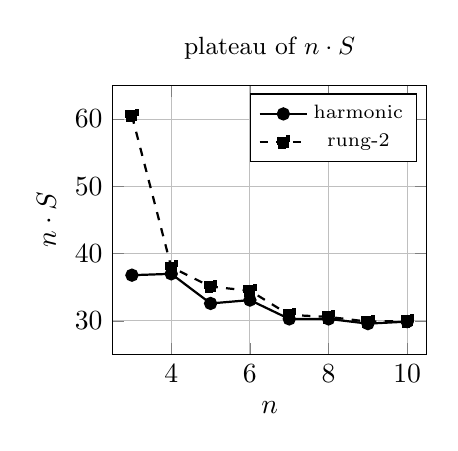
\begin{tikzpicture}
\begin{axis}[width=0.46\textwidth, height=5.0cm,
  xlabel={$n$}, ylabel={$n\cdot S$}, title={\small plateau of $n\cdot S$},
  xmin=2.5, xmax=10.5, ymin=25, ymax=65, grid=major,
  legend pos=north east, legend style={font=\scriptsize}]
\addplot[mark=*, thick] coordinates {(3,36.8)(4,37.0)(5,32.6)(6,33.1)(7,30.3)(8,30.3)(9,29.6)(10,29.9)};
\addlegendentry{harmonic}
\addplot[mark=square*, dashed, thick] coordinates {(3,60.5)(4,38.0)(5,35.1)(6,34.5)(7,30.9)(8,30.6)(9,29.9)(10,30.0)};
\addlegendentry{rung-2}
\end{axis}
\end{tikzpicture}
\hfill
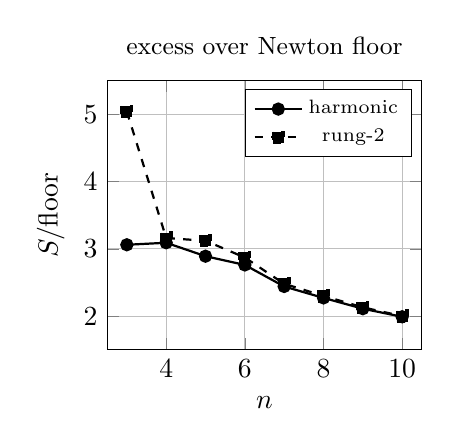
\begin{tikzpicture}
\begin{axis}[width=0.46\textwidth, height=5.0cm,
  xlabel={$n$}, ylabel={$S/\mathrm{floor}$}, title={\small excess over Newton floor},
  xmin=2.5, xmax=10.5, ymin=1.5, ymax=5.5, grid=major,
  legend pos=north east, legend style={font=\scriptsize}]
\addplot[mark=*, thick] coordinates {(3,3.06)(4,3.09)(5,2.89)(6,2.76)(7,2.44)(8,2.27)(9,2.11)(10,1.99)};
\addlegendentry{harmonic}
\addplot[mark=square*, dashed, thick] coordinates {(3,5.04)(4,3.16)(5,3.12)(6,2.87)(7,2.48)(8,2.30)(9,2.13)(10,2.00)};
\addlegendentry{rung-2}
\end{axis}
\end{tikzpicture}
\caption{The strictness records of Table~\ref{tab:hstar}. Left: the
plateau of $n\cdot S$ (the harmonic family starts at $36.8$, rung-2 at
$60.5$; both drift to $\approx30$). Right: the excess $S/\mathrm{floor}$
over the Newton floor at the minimizing coefficient---the
family-specific content of the decline---which itself decreases from
$3.06$/$5.04$ at $n=3$ to $1.99$/$2.00$ at $n=10$.}
\label{fig:nS}
\end{figure}

The two facts close the bridge in the coefficient direction, and the
falsity of the covering-radius statement (\S\ref{sec:tm-zono}) closes it
in the metric direction: the statement that strict log-concavity would
have needed to feed is false at the extremal instances, and the
coefficient structure cannot see the metric hole depth that falsifies
it. There is no mechanism, and the arithmetic is clean enough that the
absence of the mechanism is itself a datum.

\subsection{The residual question}

What survives is a question of independent arithmetic interest, and we
state it decoupled from the Lonely Runner problem entirely. The
Ehrhart data of the LR-zonotopes is governed by the gcd structure
\eqref{eq:ehr} of the projected basis; the $h^*$-polynomial of the table
is the ordinary Ehrhart $h^*$-polynomial of the lattice zonotope $Z(V)$
(its coefficients carry the gcd structure of the lattice geometry, but
the polynomial is the ordinary one---the gcd formula \eqref{eq:ehr} is
the standard zonotope Ehrhart polynomial). In every instance tested (two
core families through $n=10$, sweeps through $m\le14$ at $n=3$ and
$m\le12$ at $n=4$), the $h^*$-polynomial is real-rooted---as it must be,
by the theorem below.

\begin{corollary}\label{cor:hstarRR}
The $h^*$-polynomial of the LR-zonotope $Z(V)$ of any speed vector
$v=(v_1,\dots,v_n)$ with distinct entries and $\gcd(v)=1$---the
Ehrhart $h^*$-polynomial of the projected-basis zonotope
$\pi([0,1]^n)\subset\mathcal{X}_v$ with respect to the lattice
$\Lambda=\pi(\Z^n)\cong\Z^{n-1}$---is real-rooted.
\end{corollary}

\begin{proof}
$Z(V)=\pi([0,1]^n)$ is a lattice zonotope: a projection of the unit cube
with vertices $\pi(\{0,1\}^n)\subset\Lambda$, i.e.\ a zonotope with
integer generators $\pi(e_i)$ with respect to $\Lambda\cong\Z^{n-1}$. By
Beck--Jochemko--McCullough \cite{BJM}, the $h^*$-polynomial of every
lattice zonotope has only real roots. Hence $h^*(Z(V))$ is real-rooted.
\end{proof}

The real-rootedness is thus a special case of \cite{BJM}, and the data
of Table~\ref{tab:hstar} are a confirmation of that theorem on the
LR-zonotopes rather than a new observation. What the table records
\emph{beyond} \cite{BJM} is quantitative: the strictness $S$ (the
log-concavity margin $h_k^2/(h_{k-1}h_{k+1})$), its decay, and its
non-correlation with the covering margins---all properties of the
coefficient sequence, not of real-rootedness alone. We record the data
and do not pursue it further here: it belongs to the Ehrhart theory of
zonotopes, not to the Lonely Runner problem. It is not a bridge, and
treating it as one would repeat the pattern this paper documents.

% ======================================================================
% Appendix B — Computational provenance
% ======================================================================

\section{Computational provenance}\label{sec:prov}

The reproducibility standard of this paper is one sentence:
\emph{every number cited in the text traces to a script that was
actually run and whose output was persisted.} The standard is applied
uniformly to every cited number, inherited or new. This appendix is
the map.

\subsection{The ledger}

The provenance run (\texttt{scripts/paper\_provenance.py}; output
\texttt{out\_paper\_provenance.json} and the human-readable
\texttt{out\_paper\_provenance.txt}) reads the two persisted run records
of the zonotope program and re-asserts, by independent exact
computation, every value the paper cites from them: all witness depths
(evaluating the runner formulation \eqref{eq:runnerform} \emph{and} the
independent linear-form/lattice-search implementation, asserting exact
agreement of the two), all recorded $\rho$ values at their recorded
argmax points, all $\lambda$ and $\delta$ values, both Spearman
coefficients, both correlation instance arrays (strictness recomputed
from the Ehrhart coefficients and margins recomputed from exact
$\lambda$), and the strictness entries of the $n\le8$ table. The
complete ledger contains $225$ items. The number of failures is $0$.

The two-way witness verification deserves emphasis because it is the
strongest form of check the program has: every witness value in
Tables~\ref{tab:refute} and the fail-witness lists of
\S\ref{sec:witness} was recomputed by two implementations with different
mathematics (a one-dimensional minimization over the trajectory
parameter, and a pruned lattice search in the quotient norm's linear
forms), agreeing exactly. A one-line reproduction of the headline
witness, for the skeptical reader with the runner formulation at
hand: evaluate
$\min_\sigma\max(\wnc\sigma,\wnc{c_2-2\sigma},\wnc{c_3-3\sigma},
\wnc{c_4-4\sigma},\wnc{c_5-5\sigma})$ at
$c=(\tfrac{46}{47},\tfrac{92}{235},\tfrac{231}{235},\tfrac{35}{47})$;
the minimum is attained at $\sigma=\tfrac{4}{235}$ and the value is
$\tfrac{80}{235}=\tfrac{16}{47}$.

\subsection{The runs behind this paper}

The scripts written and run for this paper and its revisions are listed
below with their persisted outputs; the inherited records are copied
into the paper's artifact bundle.

\begin{enumerate}[leftmargin=1.6em,itemsep=2pt]
\item \texttt{hstar\_n9\_n10.py} $\to$ \texttt{out\_hstar\_n9\_n10.json}:
the $h^*$ extension of Appendix~\ref{sec:hstar} ($n=3..10$, both
families; Ehrhart asserted three ways; roots at $45$ decimal places on
exact integer coefficients; strictness, Newton, log-concavity exact;
$\lambda$ asserted against the classical values).
\item \texttt{certify\_rung2\_n5.py} $\to$
\texttt{out\_certify\_rung2.json}: the branch-and-bound certificate of
\S\ref{sec:bb}, including the cross-validation of the two $D$
implementations (forty random rational points per instance, exact
agreement), the controls ($n=3$ and $n=4$ core instances, all
certified), the negative control (harmonic $n=5$, correctly refusing),
and the ladder targets (\S\ref{sec:witness}).
\item \texttt{paper\_provenance.py} $\to$
\texttt{out\_paper\_provenance.\{json,txt\}}: the $225$-item ledger
above.
\item \texttt{certify\_followup.py} $\to$
\texttt{out\_certify\_followup.json}: the survivor enclosure analysis
of the open $m=10$ run and the recovered improved harmonic witness
($607/1792$ at $c=(\tfrac{11}{256},\tfrac{163}{256},
\tfrac{15}{256},\tfrac{79}{256})$).
\item \texttt{rho\_closeout.py} $\to$ \texttt{out\_rho\_closeout.json}:
the exact-argmax determination of the sharpest witnesses (grid and
congruence-family localization of the deepest holes, exact arrangement
analysis of the argmax regions, the binding-structure extraction of
\S\ref{sec:weights} with every binding value, translate, and
$\chi$-residual re-computed by both $D$ implementations, and the
branch-and-bound runs at the exact levels).
\item {\sloppy\texttt{closeout\_certify.py} and \texttt{lean\_closeout.py} $\to$
\texttt{out\_closeout\_*.json} and \texttt{out\_lean\_*.json}: the
two-sided close-out attempts at the exact levels: the branch-and-bound
survivor collection at the exact level (leaves certify $D\le r$ outside
the survivor boxes), the center-plus-slack Lipschitz net over the
survivors, and the exact arrangement analysis of the surviving regions
(\S\ref{sec:bb}, Table~\ref{tab:certs}).\par}
\item \texttt{m9\_witness\_hunt.py} and \texttt{m9\_ridge\_scan.py} $\to$
\texttt{out\_m9\_witness.json}: the strict $m=9$ witness of
Table~\ref{tab:refute} (multi-start exact hill-climb, then the
parametrized binding-family scan that produced the $1793/5000$ point
and its chain binding structure).
\item \texttt{local\_refine.py}: the reusable float-grid localizer used
to seed the exact arrangement analyses.
\item \texttt{certify\_m10\_v2.py} $\to$ \texttt{out\_certify\_m10\_v2.json}:
the $m=10$ close-out of \S\ref{sec:witness}: the sound multi-slice
search screen ($4.2$ million random points, dyadic grids, torsion
neighborhood, climbs, Nelder--Mead polishes, $114$ exact
re-evaluations) and the re-run branch and bound with the exact
Lipschitz box test added to the cascade ($190{,}295$ box evaluations,
$95{,}148$ certified leaves, zero survivors, $1{,}286$~s; the negative
control refusing, the $n=4$ certificates re-certifying with identical
counts, $846/846$ sampled prunes re-confirmed exactly).
\item \texttt{certify\_harmonic\_v4.py} $\to$
\texttt{out\_certify\_harmonic\_v4.json}: the harmonic close-out of
\S\ref{sec:bb}: the balance-family search (the $30{,}000$ survivor
seeds of the control run, the family witness $c(35)$, the identity
$32\,r_{(3,5)}+27\,r_{(4,5)}+35\,r_{(3,4)}=32$ verified exactly at
every member), and the branch and bound at $r=16/47$ with the
sliding-$\sigma$ gap and triple-identity certificates plus
lattice-aligned splitting at the dip lattice $q=470$ ($782{,}255$ box
evaluations, $391{,}128$ certified leaves, zero survivors, $5{,}935$~s;
$4{,}841/4{,}841$ sampled prunes re-confirmed exactly); includes the
$n=6$ $m=9$ and $m=12$ refutation searches with their exactly evaluated
dyadic witnesses.
\item \texttt{crosscheck\_cert\_witnesses.py}: the cross-validation of
the two closure runs' witness-level claims against the independent
linear-form/lattice-search implementation of this paper's ledger:
seven exact evaluations (the $m=10$ torsion center at $7/22$; the
balance family at $k=20,27,35$, each exactly $16/47$; the $m=9$ dyadic
search point at its exact depth; the $m=12$ and $m=9$ clean witnesses
at $17/47$ and $1793/5000$), zero failures, plus the binding-structure
extraction at the four $n=5$-multiple center classes (pair $(1,m)$
bisecting at each), the verification behind the archetype remark of
\S\ref{sec:weights}.
\end{enumerate}

\subsection{Certificates and budgets}

The branch-and-bound certificates are finite objects: a certificate for
$\rho(V)\le r$ is the pruned dyadic tree, each leaf carrying an exact
rational $U$-value $\le r$ computed from the kink/crossover enumeration
of \S\ref{sec:bb}. Budgets and certificate sizes for the runs cited in
the text are listed in Table~\ref{tab:certs}; the JSON persists leaf
samples, survivor aggregates (count, bounding box, maximum excess over
$r$, exact depths at sampled survivor centers), and the exact
$U$-values, so the recorded leaves and survivor aggregates can be
re-audited without re-running the search, and re-running the search
reproduces every certificate deterministically (a full leaf-by-leaf
re-audit of the largest runs requires the re-run).
The two closure runs persist, in addition, their per-certificate fire
counts (including the gap and triple-identity counts of the harmonic
cascade), the sampled-prune exact re-confirmations, and the
negative-control refusals; and their witness-level claims were
re-asserted by an independent cross-validation run
(\texttt{crosscheck\_cert\_witnesses.py}, seven exact evaluations,
zero failures) before incorporation into this paper.

\begin{table}[htbp]
\centering
\small
\caption{Branch-and-bound runs cited in the text. ``leaves'' = certified
boxes (each with exact $U\le r$, or an exact certificate of the added
Lipschitz/gap/triple-identity type); ``surv.'' = unresolved boxes at cap
or at budget; wall-clock seconds in parentheses. ``Direct closure'' =
running the tree to an empty heap at exactly $r$ with the plain
cascade; it is unavailable at non-dyadic argmaxes (\S\ref{sec:bb}),
which the plain-cascade rows record. ``Close-out'' = the two-sided
assembly of leaves, the center-plus-slack Lipschitz net, and the exact
region analyses (\texttt{lean\_closeout.py}); ``budget-open'' records
that the region analyses did not terminate within the stated budget.
The two ``certified'' rows at $r=16/47$ and at $m=10$'s $r=7/22$ are
the closures: the enhanced cascade (gap + triple-identity,
lattice-aligned splitting) and the Lipschitz box test respectively.}
\label{tab:certs}
\begin{tabularx}{\textwidth}{@{} l l >{\raggedright\arraybackslash}X r r @{}}
\toprule
instance & $r$ & verdict & leaves & surv. \\
\midrule
$(1,2,3)$ & $1/4$ & certified & $14$ $(0.0)$ & $0$ \\
$(1,2,6)$ & $3/14$ & certified & $20$ $(0.0)$ & $0$ \\
$(1,2,3,4)$ & $3/10$ & certified & $438$ $(2)$ & $0$ \\
$(1,2,3,8)$ & $5/18$ & certified & $156$ $(1)$ & $0$ \\
$(1,2,3,12)$ & $7/26$ & certified & $168$ $(1)$ & $0$ \\
$(1,2,3,16)$ & $9/34$ & certified & $222$ $(2)$ & $0$ \\
$(1,2,3,4,5)$ & $1/3$ & \emph{refused} (control) & $17{,}520$ $(421)$
& $45{,}355$ \\
$(1,2,3,4,5)$ & $16/47$ & refused (direct closure; non-dyadic argmax)
& $49{,}422$ $(3002)$ & $57{,}219$ \\
$(1,2,3,4,5)$ & $16/47$ & close-out (budget-open; $6{,}835$
net-certified, $8$ regions) & $42{,}914$ $(1400)$ & $52{,}581$ \\
$(1,2,3,4,5)$ & $16/47$ & \emph{certified} (enhanced cascade: gap +
triple-identity, lattice-aligned splitting) & $391{,}128$ $(5935)$ &
$0$ \\
$(1,2,3,4,5,12)$ & $17/47$ & refused (direct closure) & $33{,}926$
$(3004)$ & $15{,}709$ \\
$(1,2,3,4,5,12)$ & $17/47$ & close-out (budget-open; $1{,}270$
certified, $14$ regions) & $30{,}340$ $(1400)$ & $9{,}749$ \\
$(1,2,3,4,5,6)$ & $29/80$ & refused (direct closure) & $52{,}772$
$(3002)$ & $42{,}822$ \\
$(1,2,3,4,10)$ & $7/22$ & first attempt open (residual volume
$<6\times10^{-7}$) & $61{,}038$ $(1501)$ & $21{,}153$ \\
$(1,2,3,4,10)$ & $7/22$ & \emph{certified} (Lipschitz box test; sound
search screen) & $95{,}148$ $(1286)$ & $0$ \\
$(1,2,3,4,20)$ & $13/42$ & certified & $37{,}018$ $(981)$ & $0$ \\
$(1,2,3,4,25)$ & $4/13$ & certified & $10{,}414$ $(231)$ & $0$ \\
$(1,2,3,4,30)$ & $19/62$ & certified & $10{,}646$ $(274)$ & $0$ \\
\bottomrule
\end{tabularx}
\end{table}

\subsection{Reproduction}

All scripts run under CPython~3.12 with \texttt{fractions},
\texttt{numpy}, \texttt{scipy}, and \texttt{mpmath}, and take minutes
to hours on one core; the certificates of Table~\ref{tab:certs} take
seconds to minutes (the longest plain-closure certificate, $m=20$, took
sixteen minutes; the enhanced-cascade closures took twenty-one minutes
at $m=10$ and ninety-nine minutes at the harmonic instance), and the
refused control runs were run to their stated
budgets. One-line reproduction from the artifact bundle's root (each
writes its \texttt{out\_*.json} next to itself, deterministically):
\begin{itemize}[leftmargin=2.2em,itemsep=1pt,topsep=2pt]
\item \texttt{python3 hstar\_n9\_n10.py}
\item \texttt{python3 certify\_rung2\_n5.py}
\item \texttt{python3 paper\_provenance.py}
\item \texttt{python3 certify\_followup.py}
\item \texttt{python3 rho\_closeout.py} (phases: \texttt{grid47},
\texttt{tiny\_exact}, \texttt{structure}, \texttt{certify})
\item \texttt{python3 lean\_closeout.py 1,2,3,4,5 16/47} (and the
$m=12$, $m=9$, harmonic-$n=6$ analogues)
\item \texttt{python3 certify\_m10\_v2.py} and
\texttt{python3 certify\_harmonic\_v4.py} (the two closure runs)
\item \texttt{python3 crosscheck\_cert\_witnesses.py} (the
seven-witness cross-validation)
\end{itemize} The artifact
bundle accompanying the paper contains the scripts, their outputs,
the inherited zonotope records
(\texttt{out\_lrc\_zono\_final.json},
\texttt{out\_lrc\_zono\_rescan.json}, and the library
\texttt{lrc\_zono\_lib.py} they import), and the ledger. Nothing in the
paper relies on an unlogged computation, a hard-coded constant, or a
claim of the form ``verified elsewhere''.

% ======================================================================
% Appendix C — Self-contained verification core
% ======================================================================

\section{A self-contained verification core}\label{sec:self}

This appendix lets a reader with only this paper verify the sharpest
negative claims without the companion monograph. It collects the
elementary identity behind the four forms, the runner formulation with
its certificate, the explicit statement of the sum-only equality, and
one-line hand checks of the headline witnesses.

\subsection{The identity and the runner formulation}

\begin{lemma}[depth identity]\label{lem:depthid}
For every $t\in\T$,
$\max_{1\le j\le n}\wnc{\tfrac12-v_jt}=\tfrac12-\min_{1\le j\le n}\wnc{v_jt}$.
Consequently $\delta(V)=\tfrac12-\lambda(V)$ with
$\delta(V)=\operatorname{dist}_\infty\!\bigl(\R v,\;\Z^n+\tfrac12\mathbf{1}
\bigr)$, and the $\delta$-form of \S\ref{sec:prelim} is exactly
$\lrc_n$.
\end{lemma}

\begin{proof}
Each map $x\mapsto\wnc{x}$ satisfies
$\wnc{\tfrac12-x}=\tfrac12-\wnc{x}$: reflecting about $\tfrac12$
exchanges the two half-intervals and fixes the midpoint. Taking $x=v_jt$
and maximizing over $j$ gives the displayed identity (a maximum of
quantities each equal to $\tfrac12$ minus the corresponding term is
$\tfrac12$ minus the minimum). The distance form is the same statement
along the trajectory line $tv$, $t\in\R$.
\end{proof}

The computations of this paper use the \emph{runner formulation}
\eqref{eq:runnerform}, restated here:
\[
D(c)\;=\;\min_{\sigma\in[0,1)}\;\max\Bigl(\wnc{\sigma},\;
\max_{2\le j\le n}\wnc{c_j-v_j\sigma}\Bigr).
\]
Two facts make it auditable. First, it is the quotient-norm depth
$\operatorname{dist}_{\mathcal{X}_v}(c,\Lambda)$ written in the
$c$-coordinates of \S\ref{sec:prelim}: the linear forms $\phi^{1j}$,
$\phi^{ij}$ listed there generate the norm, the parameter $\sigma$ is the
free coordinate $x_1$ of a lift, and minimizing over $\sigma$ minimizes
over the lift. Second, it is \emph{Lipschitz-auditable}: each term
$\wnc{c_j-v_j\sigma}$ is $v_j$-Lipschitz in $\sigma$ and the whole
objective is piecewise linear with breakpoints at the half-integers
$c_j-\tfrac12-v_j\sigma\in\Z$, so the minimum is attained at a rational
breakpoint or crossing and is exactly computable by hand or by exact
rational arithmetic. The independent linear-form/lattice-search
implementation of the program agrees with it exactly on every instance
used in this paper (forty random rational points per instance).

\subsection{The sum-only equality, explicitly}

\begin{theorem}[sum-only equality; explicit form]\label{thm:equality-explicit}
Let $V=(v_1,\dots,v_n)$ have distinct positive entries with $\gcd(V)=1$
and $0<M(V)<\tfrac12$. For each unordered pair $\{u,w\}\subset[n]$ write
$N_{uw}=v_u+v_w$ and
\[
\tau(u,w)\;=\;\max_{0\le k<N_{uw}}\;\min_{p\in[n]\setminus\{w\}}\;
\wnc{\frac{v_pk}{N_{uw}}}.
\]
Then $M(V)=\max_{\{u,w\}}\tau(u,w)$, and consequently $\lrc_n$ holds
for all $V$ if and only if for every $V$ there is a pair $\{u,w\}$ with
$\tau(u,w)\ge 1/(n+1)$.
\end{theorem}

The two ingredients (proved in the companion monograph, Theorem~1.1
there; the finitization is what every instance of \S\ref{sec:tm-covering}
entered through) are: (i) at a global optimum $t^\ast$ with
$0<M(V)<\tfrac12$ the binding runners can be chosen two-sided---one
rising, one falling---which forces $(v_u+v_w)t^\ast\in\Z$ for that pair,
so $t^\ast$ lies on the \emph{sum} lattice of denominator $v_u+v_w$; and
(ii) on that lattice the two binding runners are exact reflections
($\wnc{v_uk/N}=\wnc{v_wk/N}$ for all $k$, since $v_u\equiv-v_w \pmod N$),
so the $n$-runner minimum equals an $(n-1)$-runner minimum. The
companion's Lemma~2.1 also records the boundary cases $M(V)=\tfrac12$
(all speeds odd) and $M(V)=0$ (impossible).

\subsection{Hand checks of the headline witnesses}

All the strict witnesses of Table~\ref{tab:refute} are one-minute hand
computations with \eqref{eq:runnerform}; the two closed values need the
branch-and-bound half of their certificates as well
(\S\ref{sec:bb}), but the witness halves are hand checks too.

\emph{The harmonic argmax value $16/47$.} Take $v=(1,2,3,4,5)$ and
$c=(\tfrac{122}{1175},\tfrac{688}{1175},\tfrac{284}{1175},
\tfrac{80}{1175})$. At $\sigma=\tfrac{96}{1175}$ (working in
$1175$-ths, with $c=(\tfrac{122}{1175},\tfrac{688}{1175},
\tfrac{284}{1175},\tfrac{80}{1175})$):
$\wnc\sigma=\tfrac{96}{1175}$;
$\wnc{c_2-2\sigma}=\wnc{\tfrac{122-192}{1175}}=\tfrac{70}{1175}$;
$\wnc{c_3-3\sigma}=\wnc{\tfrac{688-288}{1175}}=\tfrac{400}{1175}$;
$\wnc{c_4-4\sigma}=\wnc{\tfrac{284-384}{1175}}=\tfrac{100}{1175}$;
$\wnc{c_5-5\sigma}=\wnc{\tfrac{80-480}{1175}}=\tfrac{400}{1175}$.
The maximum is $\tfrac{400}{1175}=\tfrac{16}{47}$, attained twice
(runners $3$ and $5$, slopes $+3$ and $-5$ opposite), and it is
minimized: any local shift of $\sigma$ increases one of the two. Hence
$D(c)=16/47>\tfrac13=\mathrm{thr}_5$. The pair-form side of the same
point is the quadruple binding of \S\ref{sec:weights}:
$\phi^{45}(c-z)=-16/47$ at $z=(0,0,0,-1)$, $\phi^{34}(c-z)=-16/47$ at
$z=(0,1,0,0)$, $\phi^{35}(c-z)=+16/47$ at $z=0$, and
$\phi^{25}(c-z)=+16/47$ at $z=(0,1,1,1)$, each a two-term integer
evaluation.

\emph{The rung-2 argmax value $17/47$.} Take
$v=(1,2,3,4,5,12)$ and
$c=(\tfrac{4714}{5875},\tfrac18,\tfrac58,\tfrac6{25},
\tfrac{2034}{5875})$. At $\sigma=\tfrac{482}{5875}$ the six terms are
$\tfrac{482}{5875}$, $\tfrac{2125}{5875}$, $\tfrac{5693}{47000}$,
$\tfrac{13951}{47000}$, $\tfrac{1000}{5875}$, $\tfrac{2125}{5875}$:
the maximum $\tfrac{2125}{5875}=\tfrac{17}{47}$ is attained twice
(runners $2$ and $12$, slopes $+2$ and $-12$ opposite) and is
minimized, so $D(c)=17/47>\tfrac5{14}=\mathrm{thr}_6$. The binding
triple $\{2,5,12\}$ and its translates are recorded in
\S\ref{sec:weights}.

\emph{The strict witnesses.} For $v=(1,2,3,4,5,6)$ take
$c=(0,\tfrac5{16},\tfrac{15}{16},\tfrac34,\tfrac12)$ and
$\sigma=\tfrac{23}{160}$: the six terms are
$\tfrac{23}{160}$, $\tfrac{23}{80}$, $\tfrac{19}{160}$, $\tfrac{29}{80}$,
$\tfrac1{32}$, $\tfrac{29}{80}$, so $D(c)=29/80>\tfrac5{14}$ (runners
$4$ and $6$ tie at the maximum with opposite slopes). For
$v=(1,2,3,4,5,7)$ take
$c=(\tfrac1{16},\tfrac9{16},0,\tfrac38,0)$ and $\sigma=\tfrac1{11}$:
the six terms are $\tfrac1{11}$, $\tfrac{21}{176}$, $\tfrac{51}{176}$,
$\tfrac4{11}$, $\tfrac7{88}$, $\tfrac4{11}$, so $D(c)=4/11>
\tfrac5{14}$. For $v=(1,2,3,4,5,9)$ take
$c=(\tfrac1{32},\tfrac{15}{32},\tfrac{1383}{10000},
\tfrac{32921}{40000},\tfrac{95473}{200000})$ and
$\sigma=\tfrac{18577}{200000}$: the six terms are
$\tfrac{18577}{200000}$, $\tfrac{3863}{25000}$,
$\tfrac{38019}{200000}$, $\tfrac{5831}{25000}$, $\tfrac{1793}{5000}$,
$\tfrac{1793}{5000}$, so $D(c)=1793/5000>\tfrac5{14}$ (runners $5$ and
$9$ tie at the maximum).

\emph{The $7/22$ center class (the $m=10$ ladder closure's witness).}
Take $v=(1,2,3,4,10)$ and
$c=(\tfrac12,0,\tfrac12,\tfrac12)$. At $\sigma=\tfrac{7}{22}$ the five
terms of \eqref{eq:runnerform} are $\tfrac{7}{22}$, $\tfrac{3}{22}$,
$\tfrac{1}{22}$, $\tfrac{5}{22}$, $\tfrac{7}{22}$: explicitly
$\wnc\sigma=\tfrac7{22}$; $\wnc{\tfrac12-2\sigma}=\tfrac3{22}$;
$\wnc{-3\sigma}=\tfrac1{22}$;
$\wnc{\tfrac12-4\sigma}=\tfrac5{22}$; and
$\tfrac12-10\sigma=-\tfrac{59}{22}\equiv\tfrac7{22}\pmod 1$, so the
fifth term is $\tfrac7{22}$. The maximum is $\tfrac7{22}$, and it is
minimized: the binding terms are the $\sigma$-term (slope $+1$) and the
fifth term (slope $-10$), opposite signs, so any local shift of
$\sigma$ increases one of them. Hence $D(c)=7/22$, and the
branch-and-bound certificate of \S\ref{sec:bb} ($\rho\le7/22$, the
tree emptying) upgrades this to $\rho(1,2,3,4,10)=\tfrac{7}{22}$
exactly; since $\delta=1/2-\lambda=1/2-2/11=7/22$, the deepest hole at
$m=10$ is the center class itself. The pair-form side is the bisection
of \S\ref{sec:weights}: the pair $(1,10)$ binds at two translates with
opposite signs, $2\cdot 11\cdot\rho=7\in\Z$.

\emph{The balance-family witness at the harmonic argmax.} Take
$c=c(35)=(\tfrac{46}{47},\tfrac{92}{235},\tfrac{231}{235},
\tfrac{35}{47})$. At $\sigma=\tfrac{4}{235}$ the five terms of
\eqref{eq:runnerform} are $\tfrac{4}{235}$, $\tfrac{13}{235}$,
$\tfrac{80}{235}$, $\tfrac{20}{235}$, $\tfrac{80}{235}$: explicitly
$\wnc\sigma=\tfrac4{235}$;
$\wnc{\tfrac{46}{47}-2\sigma}=\wnc{\tfrac{222}{235}}=\tfrac{13}{235}$;
$\wnc{\tfrac{92}{235}-3\sigma}=\tfrac{80}{235}$;
$\wnc{\tfrac{231}{235}-4\sigma}=\wnc{\tfrac{215}{235}}=\tfrac{20}{235}$;
and $\wnc{\tfrac{35}{47}-5\sigma}=\wnc{\tfrac{155}{235}}=\tfrac{80}{235}$.
The maximum is $\tfrac{80}{235}=\tfrac{16}{47}$, attained with the
third and fifth terms binding (slopes $-3$ and $+5$, opposite), and the
tie over all three dips of the triple $\{3,4,5\}$---forced by the
identity along the family---gives the same value at every member; the
two-sided certificate of \S\ref{sec:bb} then makes $16/47$ the exact
covering radius.

Every value in
Table~\ref{tab:refute} was additionally re-asserted by two independent
implementations in the provenance run (Appendix~\ref{sec:prov}), and
the closure runs' witnesses by the cross-validation run described
there.


% ======================================================================
% Bibliography (manual, ordered by first citation)
% ======================================================================

\begingroup\sloppy\raggedright
\begin{thebibliography}{20}

\bibitem{PS-survey}
G.~Perarnau and O.~Serra,
\emph{The Lonely Runner Conjecture turns 60},
arXiv:2409.20160 (survey).

\bibitem{Wills}
J.~M. Wills,
\emph{Zwei S\"atze \"uber inhomogene diophantische Approximation von
Irrationalzahlen},
Monatsh.\ Math.\ 71 (1967).

\bibitem{Cusick1973}
T.~W. Cusick,
\emph{View-obstruction problems},
Aequationes Math.\ \textbf{9} (1973), 165--170.

\bibitem{Rosenfeld8}
M.~Rosenfeld,
\emph{The lonely runner conjecture holds for eight runners},
arXiv:2509.14111 (2025).

\bibitem{Trakulthongchai}
T.~Trakulthongchai,
\emph{Nine and ten lonely runners},
arXiv:2511.22427 (2025).

\bibitem{Sungkawichai}
T.~Sungkawichai and T.~Trakulthongchai,
\emph{Eleven, twelve, and thirteen lonely runners},
arXiv:2604.23906 (2026).

\bibitem{Allikvere}
J.~Allikvere,
\emph{Fourteen and fifteen lonely runners},
arXiv:2609.02604 (2026).

\bibitem{MSS}
R.~D. Malikiosis, F.~Santos, and M.~Schymura,
\emph{Linearly-exponential checking is enough for the Lonely Runner
Conjecture and some of its variants},
arXiv:2411.06903 (2024).

\bibitem{Rifford}
L.~Rifford,
\emph{On the time for a runner to get lonely},
arXiv:2111.13688 (2021).

\bibitem{Tao-blog}
T.~Tao,
\emph{A remark on the lonely runner conjecture},
weblog post, 13 May 2015; the observation that the optimal time is
rational with denominator the sum or difference of two speeds appears
in the comments.
\\[2pt]
\url{https://terrytao.wordpress.com/2015/05/13/a-remark-on-the-lonely-runner-conjecture}

\bibitem{prog-artifacts}
LRC reformulation program,
\emph{Companion monograph: The Lonely Runner Problem on Pair-Sum
Lattices---a lossless finitization and a conditional scaling-closure
theorem}, and the committed scripts, run logs, and experiment notes
referenced there; unpublished artifact bundle accompanying this paper
(2026).

\bibitem{BeckRobins}
M.~Beck and S.~Robins,
\emph{Computing the Continuous Discretely: Integer-Point Enumeration
in Polyhedra}, second ed.,
Undergraduate Texts in Mathematics, Springer, New York, 2015.

\bibitem{dAMoci}
L.~d'Adderio and L.~Moci,
\emph{Arithmetic matroids, the Tutte polynomial and toric
arrangements},
Adv.\ Math.\ \textbf{232} (2013), 335--367.

\bibitem{BJM}
M.~Beck, K.~Jochemko, and E.~McCullough,
\emph{$h^*$-polynomials of zonotopes},
Trans.\ Amer.\ Math.\ Soc.\ \textbf{371} (2019), 2021--2042.

\bibitem{StanleyEC}
R.~P. Stanley,
\emph{Enumerative Combinatorics, vol.~1}, second ed.,
Cambridge Studies in Advanced Mathematics 49, Cambridge Univ.\ Press,
2012.

\bibitem{Shephard}
G.~C. Shephard,
\emph{Combinatorial properties of associated zonotopes},
Canad.\ J.\ Math.\ 26 (1974), 302--321.

\bibitem{Frobenius}
G.~Frobenius,
\emph{\"Uber die Bernoullischen Zahlen und die Eulerschen Polynome},
Sitzungsber.\ K\"onigl.\ Preu\ss.\ Akad.\ Wiss.\ (1910).

\bibitem{LamLeung}
T.~Y.~Lam and K.~H.~Leung,
\emph{On the cyclotomic polynomial $\Phi_{pq}(X)$},
Amer.\ Math.\ Monthly \textbf{103} (1996), 562--564; and
\emph{On vanishing sums of roots of unity},
J.\ Algebra \textbf{224} (2000), 91--109.

\bibitem{MirskyNewman}
L.~Mirsky and D.~J.~Newman,
unpublished (the distinct-moduli theorem for exact covering systems);
the same proof was found independently by
H.~Davenport and R.~Rado,
\emph{On the density of certain sequences of integers},
J.\ London Math.\ Soc.\ \textbf{27} (1952), 224--229.

\bibitem{BrandenHuh}
P.~Br\"anden and J.~Huh,
\emph{Lorentzian polynomials},
Ann.\ of Math.\ (2) \textbf{192} (2020), no.~3, 821--915.

\end{thebibliography}
\endgroup


\end{document}
